\documentclass[12pt, a4paper, french, openright]{report}
% version reliée
% \documentclass[11pt, a4paper, french, openright, twoside]{report}
\usepackage{svg}
\usepackage{lipsum}
\usepackage[french]{babel}
\selectlanguage{french}
\usepackage[T1]{fontenc}
\usepackage[utf8]{inputenc}
\usepackage{lmodern,textcomp}

\usepackage[
    left = \flqq,%
    right = \frqq,%
    leftsub = \flqq,%
    rightsub = \frqq%
]{dirtytalk}

\usepackage{csquotes}
\usepackage{hyperref}

\usepackage{graphicx}
\usepackage[nottoc]{tocbibind}
\usepackage{caption}
\usepackage{setspace}
\usepackage{titling}
\usepackage[french,boxed,ruled,lined]{algorithm2e}

\usepackage{verbatim}
\usepackage[backend=biber]{biblatex}
\usepackage{enumitem}
\bibliography{bibliography}

\newcommand{\HRule}{\rule{\linewidth}{0.5mm}}
\renewcommand{\thefootnote}{\alph{footnote}}

\usepackage{fancyhdr}
\pagestyle{fancy}
\fancyhf{}

\renewcommand{\chaptermark}[1]{\markboth{\bsc{\chaptername~\thechapter{} :} #1}{}}
\renewcommand{\sectionmark}[1]{\markright{\thesection{} \ #1}}
\renewcommand{\headrulewidth}{0pt}
%\lhead[\textsl{\leftmark}]{\textsl{\rightmark}}
\chead[\textsl{\rightmark}]{\textsl{\leftmark}}
\cfoot[\thepage]{\thepage}
\setlength{\headheight}{15pt}

\let\headruleORIG\headrule
\renewcommand{\headrule}{\color{black} \headruleORIG}
\renewcommand{\headrulewidth}{1.0pt}
\usepackage{colortbl}
\arrayrulecolor{black}
\usepackage{tabularx}
\renewcommand{\footrulewidth}{0.4pt}% 

\usepackage{sectsty}
\usepackage{lipsum}% just to generate some text
\usepackage{glossaries}
\makeglossaries

\chaptertitlefont{\centering \MakeUppercase}




\title{Pourquoi privilégier le NoSQL au SQL dans le domaine des SIG et comment l'appliquer ?}

\author{Anthony NASCIMENTO}
\usepackage[Lenny]{fncychap}
\patchcmd{\chapter}{\thispagestyle{plain}}{\thispagestyle{fancy}}{}{}
\renewcommand\headrulewidth{0pt}
\fancyhead[L]{}
\fancyhead[C]{}
\fancyhead[R]{}
\ChNumVar{\fontsize{60}{62}\usefont{OT1}{ptm}{m}{n}\selectfont\textcolor{red}}
\makeatletter
\patchcmd{\@makechapterhead}{\vspace*{50\p@}}{\vspace*{-35\p@}}{}{}
\patchcmd{\@makeschapterhead}{\vspace*{50\p@}}{\vspace*{-35\p@}}{}{}
\patchcmd{\DOTI}{\vskip 80\p@}{\vskip 40\p@}{}{}
\patchcmd{\DOTIS}{\vskip 40\p@}{\vskip 0\p@}{}{}
\makeatother
\renewcommand\thesection{\color{red}\thechapter.\arabic{section}}

\begin{document}

\begin{titlepage}
\begin{center}

% Upper part of the page. The '~' is needed because only works if a paragraph has started.
\setlength{\parindent}{0pt}

\includesvg[width=\textwidth]{upnsvg}~\\[1cm]

%
\includegraphics[width=1\textwidth]{./upn}~\\[1cm]

\textsc{\Huge Master 2 MIAGE}\\[0.5cm]

\vspace{5mm}

\textsc{\huge \bfseries  Mémoire de fin d'études}\\[1.5cm]



% Title
\HRule

{\huge \bfseries \thetitle \\[0.4cm] }


\HRule

\vspace{5mm}

% Author and supervisor
\begin{minipage}{0.4\textwidth}
\begin{flushleft} \large
\emph{\textbf{Auteur:}}\\
Anthony \textsc{\textbf{NASCIMENTO}}
\end{flushleft}
\end{minipage}
\begin{minipage}{0.4\textwidth}
\begin{flushright} \large
\emph{\textbf{Tutrice :}} \\
Sana \textsc{\textbf{BEN HAMIDA}}
\end{flushright}
\end{minipage}

\vfill

% Bottom of the page
{\huge \bfseries Promotion 2019-2020}

\end{center}
\end{titlepage}

%page blanche
\newpage
~
%ne pas numéroter cette page
\thispagestyle{empty}
\newpage

%ne pas numéroter cette page
\thispagestyle{empty}
\begin{center}
\subsection*{Remerciements}
\end{center}


\paragraph{}Ce mémoire représente une fin en soit, la fin d'un parcours scolaire et universitaire débuté il y a vingt ans. Il représente également la fin d'une étape qui permet de continuer sur une nouvelle encore plus enrichissante.

\paragraph{}Je tiens tout d’abord à remercier Benjamin Legrand, mon tuteur de stage, et toute l'équipe de DecideOm Ile-de-France pour m’avoir accueilli, aidé et accompagné pendant toute la durée de mon stage de fin d'études.

\paragraph{}Je remercie grandement Sana Ben Hamida Mrabet pour tout le suivi réalisé durant cette année, du choix du sujet à la présentation qui accompagne ce mémoire. Je la remercie ainsi que Pascal Poizat et Sonia Guehis pour tous les conseils qu'ils ont pu me donner dans la réalisation de ce document. Je tiens également à remercier l'ensemble de l'équipe enseignante pour l'ensemble des connaissances et compétences qu'ils m'ont permis d'acquérir pendant ces trois années à Nanterre.

\paragraph{}Enfin, je remercie mes camarades de Master 2 MIAGE Mixte, spécialement Vijay Sankar, Dorian Vieira et El Hassan Baghrar et le reste de la "Team Rocket" pour les conseils qu'ils ont pu me donner. Je tenais également à saluer tous mes amis rencontrés ces trois dernières années, répartis entre toutes les MIAGE de France que j'ai pu rencontré grâce à MIAGE Connection et avec qui j'ai pu évoluer.

~
\thispagestyle{empty}

\newpage
~
\thispagestyle{empty}

\setcounter{tocdepth}{1}
\tableofcontents
\thispagestyle{empty}
\setcounter{page}{0}
%ne pas numéroter le sommaire

\newpage
~
\thispagestyle{empty}
%recommencer la numérotation des pages à "1"
\setcounter{page}{0}
\newpage

\chapter*{Introduction}
\addcontentsline{toc}{chapter}{Introduction}
\markboth{Introduction}{Introduction}
\label{chap:introduction}
\vspace{5mm}
%Pourquoi privilégier le NoSQL au SQL dans le domaine des SIG et comment l'appliquer ?
\paragraph{}75\% des applications que nous utilisons ont intégré la géolocalisation \supercite{statGeolocalisation} : de la simple cartographie aux services de transports en passant par les jeux et les réseaux sociaux, tous utilisent cette technologie. Cette fonctionnalité, parfois critiquée de par la vente des données récoltées, peut se révéler utile voire indispensable dans certaines situations. 

\paragraph{}Derrière cet outil se trouve un ensemble plus important : les\newacronym{SIG}{SIG}{Systèmes d'Information Géographiques} \gls{SIG}. Ils sont conçus pour recueillir, stocker, traiter, analyser, gérer mais également présenter les données spatiales et géographiques.

\paragraph{}La première apparition de l'analyse de données géographiques remonte à la première moitié du \textsc{xix}\ieme ~siècle dans le cadre de l'analyse d'une épidémie au sein d'un département français. Cependant, la vraie avancée dans ce domaine a eu lieu lors de la deuxième partie du \textsc{xx}\ieme ~siècle par la mise en place des premiers SIG. Depuis, la démocratisation des ordinateurs et d'Internet a permis son expansion.

\paragraph{}Les systèmes d'information sont omniprésents dans notre environnement. Qu'ils soient géographiques ou non, ils comportent un ensemble de données les permettant de fonctionner. Selon les besoins, les \newacronym{SGBD}{SGBD}{systèmes de gestion de base de données} \gls{SGBD} peuvent être relationnels ou s'éloigner de ce paradigme en utilisant du NoSQL.

\paragraph{}Pour ce mémoire, j'ai souhaité travailler autour des données, domaine qui m'intéresse surtout avec l'expension du NoSQL. Du fait qu'elles sont utilisées dans de nombreux domaines, j'ai souhaité l'affilier à un autre domaine qui m'intéresse : la géographie.

\paragraph{}Les SIG possèdent des données spatiales complétées par d'autres alphanumériques. Leur stockage est réalisé de façon à les équilibrer. Pour que ces données stockées soient utilisées de manière optimale, elles se doivent d'être modélisées auparavant. Afin de répondre à cela et aux besoins, les modèles n'ont cessé d'évoluer. Avant les années 1970, les modèles orientés texte (ressemblant aux fichiers CSV), hiérarchique et réseau étaient utilisés. Ensuite est apparu le modèle relationnel qui est aujourd'hui le plus communément utilisé à la fois dans les entrepôts de données mais également dans une partie des systèmes d'information. Ce modèle se définit par le fait qu'un ensemble de tuples ayant les mêmes attributs est appelé « relation ». Depuis, de nouveaux modèles, s'éloignant de ce paradigme, ont vu le jour avec les bases de données NoSQL : orientés objet, document, colonne ou graphe \supercite{modeles}. Selon les outils les utilisant, la modélisation des données et le modèle utilisé diffère selon les besoins.


\paragraph{}Afin de traiter le sujet, une étude sera faite sur le domaine des \acrshort{SIG}, les outils les utilisant et les modèles associés. A partir de cela, une étude comparative, basé sur plusieurs critères permettra de définir quel paradigme et quel modèle est le plus adapté pour manipuler des données géogragraphiques.
%Afin de traiter le sujet, une étude sera faite sur les différents structures et modèles utilisés par les différents outils que nous connaissons. A partir de cela, nous pourrons établir les critères permettant de choisir le modèle de données le plus adéquate que nous appliquerons à un exemple.





\chapter{Le NoSQL dans les SIG}

\section{Les Systèmes d’Information Géographiques}
\subsection{Définition}
\paragraph{}Un système d'information géographique est un système d’information permettant, à partir de plusieurs sources de données, de recueillir, stocker, traiter, analyser, gérer et présenter des données à la fois spatiales et géographiques. Les \acrshort{SIG}, avec d’autres traitements, font partie du domaine de la géomatique. 

\paragraph{}Comme tout système d’information, le \acrshort{SIG} offre un soutien aux processus de travail. Il permet d'analyser spatialement un phénomène tout en fournissant l'information et automatisant le travail humain.

\subsection{Historique}
\paragraph{}Les années 1960 correspondent au début des \acrfull{SIG}. Avec l’apparition des ordinateurs, les premiers travaux de recherches sont apparus sur des sujets comme l’analyse spatial et la visualisation de l’information géographique, constituant donc les bases des \acrshort{SIG}. Auparavant, diverses analyses spatiales ont pu être effectuées en France ou au Royaume-Uni comme celle concernant les effets du choléra dans l’ancien département de la Seine \footnote{ancien département comprenant Paris et une partie des communes des Hauts-de-Seine, de Seine-Saint-Denis et du Val-de-Marne} en 1832 \supercite{rapportCholeraSeine}. Toutefois, c’est le développement de l’informatique dans la deuxième partie du XXème siècle qui a permis le développement des \acrshort{SIG} en tant que tel.
\paragraph{}En 1963, Robert Tomlinson \supercite{tomlinson} a mis en place un outil permettant de regrouper des données sur l’inventaire des ressources naturelles et sols canadiens et cela constitue le premier \acrshort{SIG}. En parallèle, Howard Fisher a créé le premier logiciel de cartographie informatique, nommé SYMAP. En 1965, il crée le Laboratoire de Harvard pour l'infographie et l'analyse spatiale où seront conçus les premiers concepts et applications dans ce domaine. Ces recherches ont permis le développement de systèmes dans les années 1970, utilisés par les universités, les centres de recherche et des entreprises.

\paragraph{}Le \acrshort{SIG} canadien a servi de base de travail jusqu’en 1986 où le premier \acrshort{SIG} à usage personnel a été créé : le système MIDAS (Mapping Display and Analysis System). Par la suite, le développement à la fois des systèmes d’information et d’Internet ont permis la démocratisation des \acrshort{SIG}. C’est à ce moment, en 1994, que l’Open Geospatial Consortium a été créé par promouvoir des standards liés à l’information géographique et la géomatique afin de permettre l’interopérabilité des contenus et échanges. Plus récemment, les solutions Open Source ont permis de rendre ces technologies plus accessibles.

\paragraph{}Depuis, nombre d'entre eux sont utilisés dans divers domaines allant de la cartographie avec les services de géolocalisation à l'analyse de situations telles que les élections, les déplacements de populations ou les épidémies à l'instar des outils réalisés suite à la pandémie de COVID-19 :
\begin{figure}[htp]
  \centering
  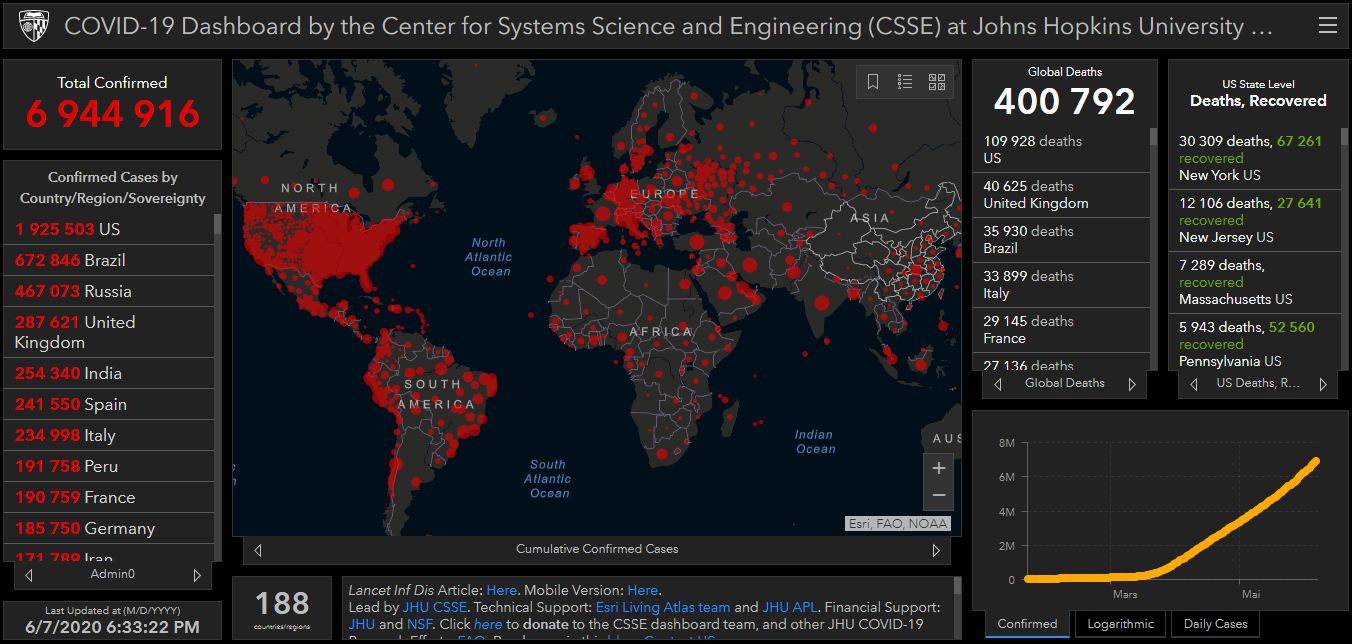
\includegraphics[width=120mm]{src_img/gis_use_example.png}
  \caption{Utilisation d'ArcGIS (un \acrshort{SIG}) dans le cadre de l'épidémie de Covid-19\supercite{arcgisCovid}}
  \label{fig:arcgisexemple}
\end{figure}

\subsection{Les composants}
Pour réaliser tout ce qui lui est induit, les systèmes d’information géographiques sont composés \supercite{giscomponents} de :
\begin{description}
    \item[matériel informatique :] les \acrshort{SIG} fonctionnent sur une large gamme de matériel, de serveurs informatiques centralisés aux ordinateurs de bureau utilisés dans des configurations autonomes ou en réseau
    \item[logiciels :] ils fournissent les outils nécessaires pour sauvegarder, traiter et visualiser l’information géographique contenue dans des bases de données
    \item[données :] l’information géographique est la pièce maîtresse des \acrshort{SIG}. Elle peut être récupérée ou constituée
    \item[personnel :] les outils nécessitent des personnes chargées de manipuler et traiter l’information géographique. La démocratisation des \acrshort{SIG} a permis l’augmentation du nombre d’utilisateurs
\end{description}

\subsection{Les principes des SIG}

Ces composants ensemble permettent de suvre les principes des “5A” :
\begin{description}
    \item[L’acquisition :] Elle correspond à obtenir et regrouper différentes sources afin de les intégrer au SIG selon le problème à résoudre. Les sources sont diverses (visites de terrain, satellite, etc.)
    \item[L’archivage :] Consiste à réaliser un choix concernant le stockage et le traitement des données, organisé par thématique (ex: voirie, occupation des sols)
    \item[L’accès :] Mise à disposition des données d’information (données et cartes) et de les combiner
    \item[L’analyse :] Correspond aux possibilités offertes par le SIG pour traiter les données au travers d’outils grâce à des mesures, des calculs ou des requêtes spatiales
    \item[L’affichage :] Correspond en la restitution cartographique des données correspondant au besoin spécifique
\end{description}

\paragraph{}Un sixième aspect est également parfois cité, l’abstraction \supercite{courssig}. Cet aspect correspond à permettre la conception d'un modèle arrangeant les données par constituants géométriques et attributs descriptifs tout en établissant les relations entre les objets.


\subsection{Les données}
Les \acrshort{SIG} se basent sur deux types de données qui se complètent : spatiales et attributaires.

\subsubsection{Données spatiales}

Un Système d’information Géographique s’appuie sur un modèle de couches organisé de manière cohérente afin de décrire et caractériser le plus fidèlement le monde. Par exemple, un SIG peut avec comme couches la topologie \footnote{étude des déformations du sol}, les réseaux hydrographiques ou de communication ou le découpage et l'occupation des sols.

Deux formats permettent de stocker les données spatiales (99\% des SIG savent traiter les deux types) :

\begin{itemize}[label=\textbullet]
    \item Le format raster, ou maillé, a une géométrie fondée sur un découpage en mailles élémentaires, de la même façon qu’une image numérique est découpée en pixels. L’information spatiale apparaît sous la forme d’un tableau de valeurs numériques référencées géographiquement.
    \item Les vecteurs ont une géométrie fondée sur un système de coordonnées vectorielles assimilables au dessin classique d’une carte traditionnelle. Les objets spatiaux sont représentés par des points, des arcs ou des polygones, et la position des objets est donnée par rapport à un repère standard (géographique ou cartésien).
\end{itemize}
\begin{figure}[htp]
  \centering
  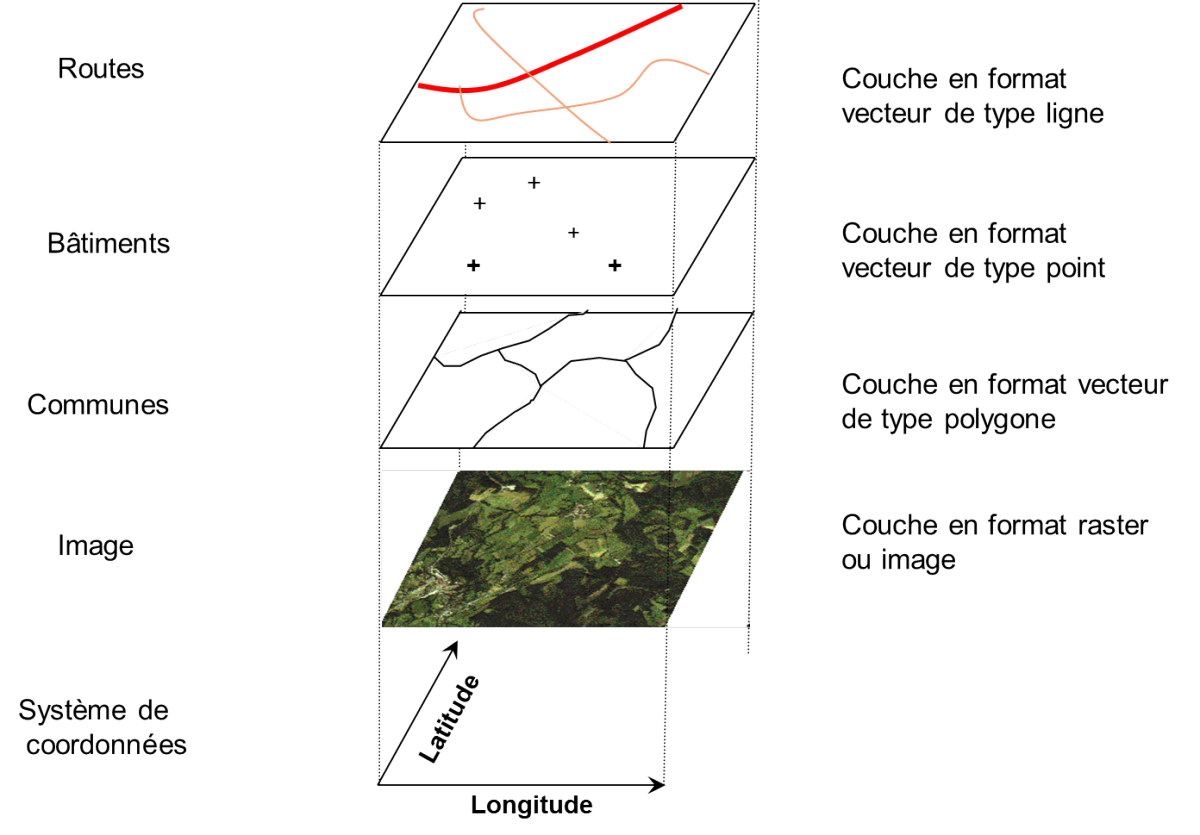
\includegraphics[width=90mm]{./src_img/structure_donnees.png}
  \caption{Exemple de couches \supercite{uved}}
  \label{fig:struct}
\end{figure}
Comme il est possible de voir sur le schéma de la figure \ref{fig:struct}, la représentation d'une situation géographique correspond souvent à l'utilisation des deux formats présentés. Pour leur stockage, il est réalisé par le biais d'arbres et de graphes \supercite{arbresSIG} qui permettent d'équilibrer les données.

%Sur l'exemple ci-dessus (figure \ref{fig:struct}), les différentes couches et formats présentés juste avant.

%Les SIG possèdent des données spatiales qui peuvent être stockées soit en format vectoriel, soit en format raster. Le vectoriel va gérer les points, les lignes et les polygones alors que le raster va utiliser une photographie aérienne, une carte ou une image satellite pour la découper sous forme d'une matrice. Cette matrice de cellules (ou pixels) est elle-même organisée sous forme de grille. Ces données spatiales, qu'elles soient sous format vecteur ou raster, sont complétées par des données alphanumériques. Leur stockage est réalisé avec l'utilisation d'arbres et de graphes \supercite{arbresSIG} qui permettent d'équilibrer les données.
%Par exemple, un SIG peut distinguer parcelles, images satellites, réseau hydrographique et bâtiments sur une zone d’intérêt.

\subsubsection{Données associées}
\paragraph{}Ces données permettent, avec la topologie \footnote{topologie : décrit les relations entre objets}, de compléter l’information spatiale \supercite{courssig2} comme il est possible de voir dans la figure \ref{fig:besoinSpatial}. Elles constituent en quelque sorte l’étiquette permettant de donner des détails sur un point, une ligne ou un polygone. Parmi les données associées :
`\begin{itemize}[label=\textbullet]
    \item les données de classification : elles permettent de classer la forme selon des classes déterminées, par exemple si une route est primaire ou secondaire ou si une parcelle est irriguée ou non
    \item les données d’identification : ce sont les informations distinguant un objet d’un autre comme le nom de la commune, le numéro de parcelle
    \item les données attributaires  : c’est une information complémentaire propre à l’objet (ex : propriétaire, superficie)
\end{itemize}

\begin{figure}[htp]
  \centering
  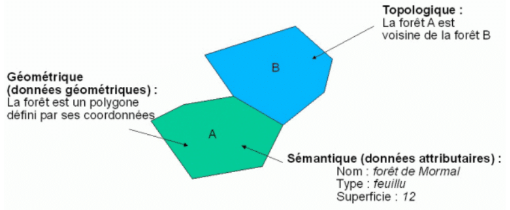
\includegraphics[width=95mm]{src_img/exempleBDS.png}
  \caption{Les 3 niveaux de la donnée géographique \supercite{ensg}}
  \label{fig:besoinSpatial}
\end{figure}

\section{Quelles différences entre SQL et NoSQL ?}

\subsection{Les bases de données relationnelles}

\paragraph{}Les bases de données relationnelles utilisent un modèle établit par Edgar F. Codd en 1970. Dans ce modèle, l’information est organisée dans des tableaux à deux dimensions, appelées relations ou tables et faisant correspondre ces données selon des caractéristiques communes. Chaque table est donc structurée par un schéma préconçu.

\paragraph{}Codd a également établit le langage\newacronym{SQL}{SQL}{Structured Query Language} \acrshort{SQL}, permettant de créer le schéma et les données mais également d’interroger la base de données, y compris des opérations d’intersection, de sélection ou de jointure. Il est utilisé par les différents \acrlong{SGBD} relationnels tels que Oracle, Sybase, Microsoft SQL Server ou Access.

\subsubsection{Propriétés}
\paragraph{}Les SGBD relationnels suivent les propriétés ACID :
\begin{description}
    \item[Atomicité :] signifie «tout ou rien». Si une partie de la transaction reste incomplète, la transaction entière est considérée comme ayant échoué.
    \item[Cohérence:] garantit qu'une base de données avant et après toute transaction est stable à un état valide.
    \item[Isolation:] garantit que plusieurs transactions exécutées en même temps n'affectent pas l'exécution de l'autre, cela nécessitant la sérialisation des transactions simultanées
    \item[Durabilité:] garantit qu'une fois qu'une transaction a été validée, elle reste dans le même état, c'est-à-dire qu'elle stocke en permanence même en cas d'erreurs, de panne du système ou de coupure de courant
\end{description}

\subsection{Les bases de données NoSQL}

\paragraph{}Les bases de données NoSQL (“Not only SQL” ou “pas seulement SQL”) sont apparus à la fin des années 2000 avec le développement des centres de données et la nécessité d’avoir un paradigme adapté à une architecture en clusters, donc distribuée. Cette architecture apporte aussi la possibilité d’accès et modifications concurrentes, non permises par les propriétés ACID des SGBD relationnels. Elle est également auto-descriptive et ne nécessite donc pas de schéma.

\paragraph{}Afin de répondre à des volumes de plus importants (comme le Big Data) et leur besoin de gérer des données distribuées, certaines entreprises du web ont créé leurs propres \acrshort{SGBD} : BigTable pour Google, MongoDB sur SourceForge.net et Cassandra puis HBase pour Facebook. Ces solutions sont devenus de plus en plus adoptées lors de la dernière décennie. 

\subsubsection{Propriétés}
\paragraph{}Associé au développement des systèmes distribués, un nouveau concept opposé à ACID est apparu, le concept BASE :
\begin{description}
    \item[Basic Availability :] le système doit à tout moment  être accessible.
    \item[Soft state :] l'état de la base de données n'est pas garanti à un instant t.
    \item[Eventually Consistent :] la cohérence des données à un instant t n'est pas primordiale.
\end{description}

\subsubsection{Diffférents modèles existants}
\begin{description}
    \item[Clé-valeur \supercite{NoSQLModels} :] le modèle de données basé sur un tableau associatif dans lequel les données sont représentées sous une collection de paires clé-valeur. Ils conviennent parfaitement à la gestion de session et à la mise en cache dans les applications Web (utilisé par LinkedIn)\\
    Exemples: Aerospike,  Redis, Riak\\
    \item[Colonne :] une large colonne stocke et organise les tableaux de données sous forme de colonnes plutôt que de lignes. Cette structure permet d’interroger rapidement un grand volume de données comme pour les moteurs de recommandation, les catalogues, la détection de fraude, etc. (Utilisé par Amazon, Google et Facebook) \\
    Exemples: Cassandra, HBase, Google BigTable\\
    \item[Document :] ce modèle conserve les données semi-structurées ainsi que leur description au format du document (souvent XML ou JSON). Chaque document possède une clé unique à travers laquelle il est adressé. Ils sont particulièrement pour la gestion de contenus et de données des applications mobile mais avec JSON et lors d’utilisations d’API. (Utilisé par Expedia, SAP et Salesforce) \\
Exemples: Apache, MongoDB, CouchDB, BaseX\\
    \item[Graphe :] les données sont organisées en nœuds (correspondant à un enregistrement) et en arêtes. Ce modèle prend en charge une représentation plus riche des relations de données. Ils sont utiles pour les systèmes de gestion de la relation client, les cartes routières, les systèmes de réservation, etc. (Utilisé par eBay et Accenture)\\
Exemples: AllegroGraph, InfiniteGraph,  Neo4j, Titan\\
\end{description}
\subsection{Des possibilités d'analyse sur plusieurs dimensions}
Nous avons pu voir que le choix de la structure est primordial dans la mise en place d'une base de données. Il est également nécessaire de penser à l'analyse qu'on ferait de son contenu. Pour répondre à des besoins de plus en plus importants concernant l'analyse sur plusieurs thématiques à la fois, l'analyse multidimensionnelle a été mise en place, en particuliers avec les technologies OLAP \footnote{OnLine Analytical Processing}.

\begin{figure}[!htp]
  \centering
  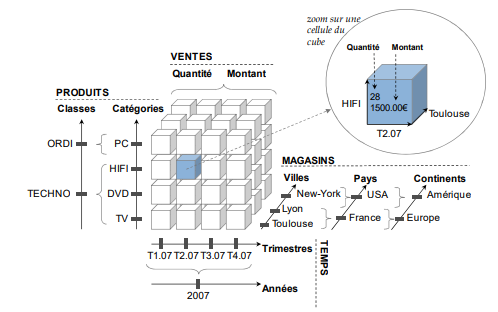
\includegraphics[width=75mm]{./src_img/exempleOLAPCube.png}
  \caption{Exemple de cube OLAP\supercite{tel-01456620}}
  \label{fig:olapcube}
\end{figure}

\paragraph{}Nous pouvons voir avec le cube de la figure \ref{fig:olapcube} qu'une des dimensions concerne des données géographiques, les villes. Le cube permet, par des opérations simples que sont le "drill-up" et le "drill-down" de remonter ou descendre la hiérarchie d'une dimension, par exemple accéder au niveau régional ou national des données.

\paragraph{}Toutefois, pour obtenir un cube que celui-là, il faut travailler à la conception de l'entrepôt de données dans lequel sont basées toutes les informations que l'on souhaite utiliser. Trois modèles existent dont un qui reprend les précédents :
\begin{itemize}[label=\textbullet]
    \item le modèle en étoile (figure \ref{Fig:modeletoile}) : il comprend une table de fait centrale avec des mesures qui sont dépendantes des différentes dimensions autour. Souvent sont utilisées une dimension géographique et une dimension temporelle
    \item le modèle en flocon (figure \ref{Fig:modelflocon}) : tout comme le modèle en étoile, il comprend une table de fait et des dimensions mais à l'instar d'un flocon de neige, ces dimensions ont des ramifications avec les hiérarchies sous-jacentes
    \item le modèle en constellation : il reprend les principes soit du modèle en étoile, soit du modèle en flocon mais à la différence qu'il comprend plusieurs tables de faits
\end{itemize}
\begin{figure}[!htb]
   \begin{minipage}{0.48\textwidth}
     \centering
     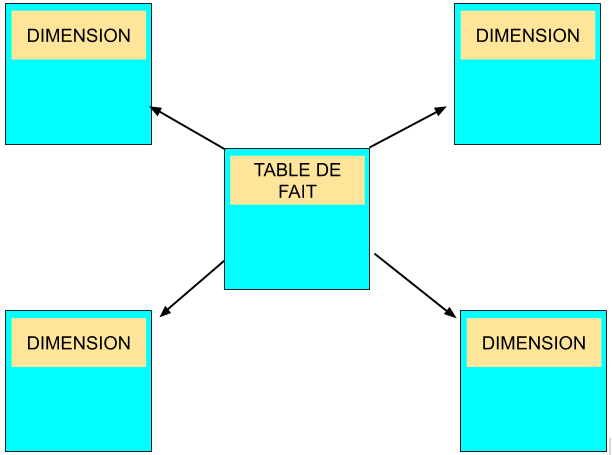
\includegraphics[width=.6\linewidth]{./src_img/Star-schema.png}
     \caption{Modèle en étoile}\label{Fig:modeletoile}
   \end{minipage}\hfill
   \begin{minipage}{0.48\textwidth}
     \centering
     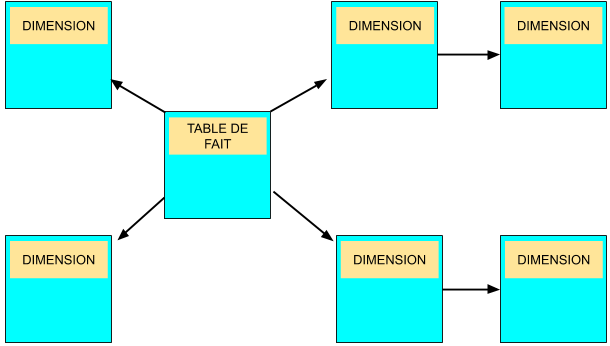
\includegraphics[width=.7\linewidth]{./src_img/SnowFlake-schema.png}
     \caption{Modèle en flocon}\label{Fig:modelflocon}
   \end{minipage}
\end{figure}
\paragraph{}Le modèle en étoile a par exemple l'avantage de permettre des requêtes plus simples, d'améliorer des performances des requêtes et l'alimentation d'un cube OLAP dont cette structure est privilégiée. A l'inverse, le modèle en flocon  permet d'avoir une structure plus normalisée  qui facilite donc l'ajout et surtout la mise à jour. En prenant l'exemple de la figure \ref{fig:olapcube}, les 2 modèles sont possibles. Cependant, pour l'utilisation d'un cube OLAP, le modèle en étoile est à privilégier.

Dans le cadre du NoSQL, à partir d'un document, d'une grosse colonne, plusieurs méthodes permettent de traduire la structure de données  \supercite{sgbd} :
\begin{itemize}[label=\textbullet]
    \item la traduction plate : l'ensemble des attributs de mesures et dimensions sont dans un même document
    \item la traduction par imbrication : les attributs et dimensions sont embriqués par catégorie dans le document
    \item la traduction hybride : les attributs et dimensions sont dans des documents différents avec des références entre eux
    \item la traduction éclatée : les attributs et dimensions sont dans des documents différents eux mêmes compris dans des collections
\end{itemize}
\paragraph{}Cette transformation permet ensuite une meilleure adaptabilité pour une utilisation dans un cube OLAP.

\subsection{Enoncé des différences notables}
\paragraph{}De nombreuses différentes entre SQL et NoSQL, à prendre à compte dans le choix d’un \acrshort{SGBD}. Les quatres principales distinctions sont :

\subsubsection{Le langage}
\paragraph{}Les SGBDR possèdent le SQL comme langage de requêtage. Sa structure, composée de schémas prédéfinis nécessite de déterminer la structure des données et donc une préparation initiale. Toutefois, cette structuration lui permet de mieux gérer les requêtes complexes. De leur côté, les bases de données NoSQL disposent d’un schéma dynamique. Cependant, les requêtes se basent sur \newacronym{UnQL}{UnQL}{Unstructured Query Language} \gls{UnQL} dont la syntaxe varie d'une base de données à l'autre.

\subsubsection{L’évolutivité}

\paragraph{}Dû à son architecture, les bases de données NoSQL peuvent plus facilement évoluer que les SQL et faire face à une augmentation du trafic. En effet, les SGBD relationnels, évolutifs verticalement, nécessitent d’augmenter la charge d’un seul serveur en augmentation ses composants (RAM, SSD, CPU) alors que le NoSQL nécessite uniquement l’augmentation du nombre de serveurs. De cette façon, le NoSQL est également plus résistant aux pannes et coûte donc moins cher \supercite{costNoSQL}. Par ailleurs, le schéma fixe rend plus difficile l’évolution en fonction des besoins de l’entreprise dans les SGBD SQL car les changements de schéma sont problématiques et prennent du temps.

\subsubsection{La communauté}
\paragraph{}Le langage SQL, créé en 1974, a acquis une certaine maturité au fur et à mesure des années, augmentant donc sa communauté. Cette popularité est présente via les nombreux forums existants permettant ainsi d’améliorer les compétences. En revanche, bien que NoSQL se développe rapidement, il est relativement nouveau et donc sa communauté n’est pas aussi bien définie.

\subsubsection{La structure}
\paragraph{}Les bases de données SQL utilisent des relations et est particulièrement adéquate pour des systèmes ayant des structures bien définies alors que dans les NoSQL, les données peuvent être stockées suivant différents modèles (document, graphe, …) et la structure, propre à chaque document, offre donc plus de libertés.

\paragraph{}Parmi les autres éléments qui peuvent être cités, les SGBD NoSQL sont plus que adaptés au Big Data du fait qu’ils ont été créés pour gérer de grandes quantités de données, ce qui permet d’avoir des temps d’exécution beaucoup plus rapides \supercite{comparatifmongomysql}. Cependant, les SGBD relationnels sont plus sécurisés à la fois pour l’authentification, la confidentialité et les communications \supercite{serveyNoSQL}.

\begin{table}[h!]
\begin{tabularx}{\textwidth} { 
  | >{\centering\arraybackslash}X 
  | >{\raggedright\arraybackslash}X 
  | >{\raggedright\arraybackslash}X | }
 \hline
\rowcolor{lightgray}
 \textbf{Critère} & \textbf{SQL} & \textbf{NoSQL} \\
 \hline
 Langage de requêtage  & SQL   & Syntaxe variable mais basée sur UnQL  \\
\hline
 Structure  & Prédéfini et travaillé en amont   & Dynamique  \\
\hline
 Évolutivité  & Verticale \newline Augmentation de ressources  & Horizontale \newline  Augmentation du nombre de serveurs \\
\hline
 Communauté  & Large  & Pas encore bien définie  \\

\hline
\end{tabularx}
\caption{Synthèse}
\end{table}

\section{Pourquoi privilégier le NoSQL dans les SIG ?}

\subsection{Le SGBDR avec des performances limitées}

\paragraph{}Actuellement, les systèmes de gestion de bases de données relationnels restent majoritairement utilisés dans l’univers des SIG dû à la récence du NoSQL. De ce fait, nombre d’entre eux utilisent encore les propriétés ACID. Quand le projet nécessite que peu de données géographiques, une base de données NoSQL n’est pas nécessaire. Cependant, quand il nécessite de gérer une grosse volumétrie, la réflexion peut s’amener.
\paragraph{}Plusieurs SGBDR ont mis en place des modules ou outils spécialement dédiés aux SIG pour faire face à la demande. Des études ont déjà été réalisées pour comparer d’une part l’un d’entre eux à un NoSQL de l’autre. Par exemple, dans une étude comparant DocumentDB, orienté document comme son nom le dit, avec Azure SQL DataBase\supercite{azuredocumentdb}, il s’est révélé que grâce à son architecture distribuée, DocumentDB gère mieux le partage des ressources et est également plus rapide. Cependant, grâce à ses propriétés ACID, Azure SQL Database gère mieux les demandes simultanées avec un meilleur taux de succès.

\subsection{Une architecture plus favorable à l’explosion des données}

\paragraph{}Ces dernières années, le volume d’informations traités par l’ensemble des systèmes d’information a explosé. Le trafic généré comprend 80\% de données non ou semi-structurées qui nécessitent d’être traités par des systèmes dédiés. C’est également le cas des données géographiques utilisées pour la géolocalisation, l’IOT, la gestion des ressources naturelles, etc. 

\paragraph{}L’importante quantité de données nécessitent d’avoir les ressources matérielles adéquates. Les SGBDR permettent la montée d’un seul serveur. Cependant, ceux-ci ont une certaine limite qu’il ne peuvent dépasser. Au-delà, les bases de données SQL ne sont plus adaptées et il est nécessaire d’opter pour une autre architecture, cette fois-ci distribuée comme l’est le NoSQL. Une architecture comme cela aura donc plusieurs avantages :
\begin{itemize}[label=\textbullet]
    \item une meilleure scalabilité : on peut augmenter le nombre de serveurs pour faire face à la montée en charge
    \item une résistance aux pannes : si un serveur tombe en panne, le service ne sera pas inaccessible contrairement à une architecture centralisée car la réplication assurera la présence de sauvegardes sur les autres serveurs
\end{itemize}


\paragraph{}Le NoSQL est également plus adapté pour une utilisation sur un Cloud et est aussi plus favorable pour la mise en place de DBaaS (Database As A Service) pour des besoins de scalabilité et de haute disponibilité.

\subsection{Une meilleure adaptabilité aux divers formats de données}
Comme évoqué auparavant, la structure des données dans les SIG n’est pas uniforme avec les mêmes propriétés pour tout élément. Les données géographiques sont une combinaison de plusieurs informations : les données spatiales correspondant aux différentes couches et entités de l’environnement et les données associées aux données spatiales et donnant plus de détails sur celles-ci.


\chapter{Panorama des solutions industrielles}
\paragraph{}Nosu avons pu voir pourquoi il est préférable de privilégier le NoSQL au SQL pour la gestion des données géographiques, notamment au sein des \acrshort{SIG}. Pour compléter cela, nous allons faire un tour des solutions existantes que nous allons comparer selon des critères prédéfinis. Nous commencerons par un outil liés au relationnel pour avoir un regard sur ce qu’il existe. Nous passerons ensuite sur des SGBD NoSQL intégrant des modules liés aux SIG puis enfin SOLAP, un des outils les plus adaptés à l’analyse spatiale.

\section{Les critères de comparaison}

\paragraph{}Afin de pouvoir évaluer correctement chacune des solutions, il est primordial de définir des critères qui nous permettront de les comparer.

Nous avons pu voir pourquoi privilégier le NoSQL au SQL pour la gestion des données géographiques au sein des SIG. Pour compléter cela, nous aurons un tour d’aperçu des différentes solutions dans ce domaine. 

\subsubsection{Catégorie 1 : les caractéristiques du SGBD}
Ces critères, propres à chaque SGBD, seront étudiés à la fois dans la présentation des outils mais également dans l'application.
\begin{enumerate}
    \item \textbf{Le type} \\ Le \acrshort{SGBD} respecte-il les règles de Codd ou sort-il de ce paradigme ? \newline
    \item \textbf{Le schéma} \\ Le \acrshort{SGBD} permet-il un schéma fixe ou libre ? \newline
    \item \textbf{Le modèle} \\ Quel modèle est utilisé ? \newline
    \item \textbf{Le langage de requêtage} \\ Quel est le langage de requêtage principalement utilisé pour rechercher ou traiter des données ?
\end{enumerate}

\subsubsection{Catégorie 2 : les comparaisons dans l'implémentation de la base}
Ces critères permettant de comparer les bases de données seront étudiés dans l'application. Ils permettront d'évaluer l'occupation et l'implémentation des modèles.
\begin{enumerate}
    \item \textbf{Taille occupé par la base} \\ Quel est l'espace occupé ? \newline
    \item \textbf{Le nombre d'objets} \\ Combien d'objets sont contenus dans la base ? \newline
\end{enumerate}


\subsubsection{Catégorie 3 : l'exécution de la requête}
Ces critères permettant de comparer les bases de données seront étudiés dans l'application. Ils auront pour but de comparer les résultats fournis par les différents SGBD.
\begin{enumerate}
    \item \textbf{Temps d'exécution} \\ Quel temps a été utilisé pour réaliser la requête associée \newline
    \item \textbf{Nombre de résultats} \\ Nombre de tuples affichés \newline
    \item \textbf{Nombre d'objets manipulés} \\ Combien d'objets ont-ils été manipulés et lus pour répondre à la requête ?
\end{enumerate}


%Critères 
%standards : langage, modèle, type
%calculs : temps d'exécution, nb d'objets sollicités

\section{Des extensions SIG dans les SGBD relationnels}

\subsection{Les bases de données spatiales}

\paragraph{}Parmi toutes les informations qui circule dans le monde, 80\% ont un caractère spatial et nécessite des bases de données adaptées pour son traitement. L’architecture liée aux SIG a évolué au fur et à mesure des années : la première génération était centrée sur les outils avec un stockage dans les systèmes de fichiers, la deuxième était hybride mélangeant données SIG et attributaires et enfin la troisième et actuelle génération intègre données géométriques et attributaires sous un même schéma. Ceci facilite l’interaction entre les différents types de données. Différents types existent :
\begin{figure}[htp]
  \centering
  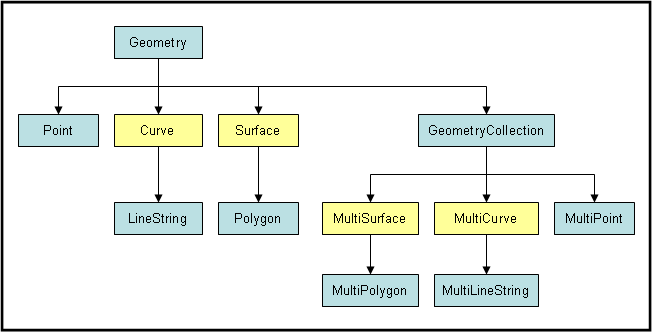
\includegraphics[width=140mm]{src_img/geometryhierarchy.png}
  \caption{Hiérarchie géométrique \supercite{hierarchygeo}}
  \label{fig:geometryHierarchie}
\end{figure}

\paragraph{}Comme le montre la figure \ref{fig:geometryHierarchie}, la géométrie d'un objet peut avoir plusieurs configurations : sous forme de point, de ligne ou de polygone. Cependant, chacun d'entre eux n'ont pas les mêmes propriétés, ils ne peuvent pas se retrouver dans une même table en suivant les standards relationnels. Nous aurons par exemple une table pour les limites de territoires (région, ville, quartier), une autre pour la topographie \footnote{topographie : relief d'un lieu} et une autre pour les données hydrographiques.

\paragraph{}Cette configuration par l'utilisation d'objets est l'un des principes mis en place par\newacronym{OGC}{OGC}{Open GeoSpatial Consortium} l’\acrfull{OGC} afin de permettre l'interopérabilité.


%\paragraph{}Comme nous pouvons le voir, les points, lignes et polygones caractérise l’aspect spatial des données mais n’ont pas le même standard au niveau SQL. En effet, chacun des objets ayant ses caractéristiques propres, elle ne peuvent être dans une même table : par exemple, une pour les limites d’une ville, une pour la topologie \footnote{Étude des déformations du sol}, une pour les données hydrographiques, etc. Cependant, \newacronym{OGC}{OGC}{Open GeoSpatial Consortium} l’\acrfull{OGC} a mis en place un certain nombre de principes pour permettre l’interopérabilité.

\subsection{Une large gamme de choix d'outils spatiaux relationnels}

\paragraph{}Dans les SIG intégrant des bases de données relationnelles, nous avons deux catégories.

\subsubsection{Les fonctions spatiales sur les SGBD traditionnels}
\paragraph{}Un certains nombre d'éditeurs de \acrlong{SGBD} ont mis en place au sein de leurs outils des extensions permettant à la fois de stocker et de réaliser des opérations sur des données spatiales. C'est le cas par exemple de MySQL, PostGreSQL et SQLite qui ont respectivement proposé MySQLSpatial, PostGreSQL et SpatiaLite. SAP HANA, Oracle Spatial, Microsft SQL Server ou DB2 sont également d'autres exemples de \acrshort{SGBD} relationnels qui offrent la possibilité de réaliser des requêtes spatiales.


%\paragraph{}Nous avons d'abord un certain nombre d'éditeurs de SGBD qui ont mis en place des extensions permettant de stocker et réaliser des opérations sur des données spatiales. C'est par exemple le cas de MySQL avec MySQL Spatial, PostGreSQL avec PostGIS et SQLite avec SpatiaLite. SAP HANA, Oracle Spatial, Microsft SQL Server ou DB2 sont d'autres exemples de systèmes de gestion de bases de données qui offrent la possibilité de réaliser des requêtes spatiales
\subsubsection{Les SIG intégrant les principes relationnels}
\paragraph{}La deuxième catégorie est celle des SIG intégrant eux-mêmes une lecture ou un stockage de données organisées de manière relationnelles. QGis intègre par exemple l'extension spatiale de PostGIS tout en permettant la gestion des données vectorielles. CARTO, un service de cartographie, aussi intégre la même extension.

%\paragraph{}Dans les SIG intégrant des bases de données relationnelles, nous avons deux catégories. Nous avons d'abord un certain nombre d'éditeurs de SGBD qui ont mis en place des extensions permettant de stocker et réaliser des opérations sur des données spatiales. C'est par exemple le cas de MySQL avec MySQL Spatial, PostGreSQL avec PostGIS et SQLite avec SpatiaLite. SAP HANA, Oracle Spatial, Microsft SQL Server ou DB2 sont d'autres exemples de systèmes de gestion de bases de données qui offrent la possibilité de réaliser des requêtes spatiales



\paragraph{}Pour notre étude, nous allons nous concentrer sur PostGIS, un des outils les plus présents dans ce domaine et nous allons donc le découvrir un peu plus en profondeur.

%\paragraph{}Un certain nombre d’éditeurs de SGBD relationnels ont mis en place des extensions spatiales parmi lesquels MySQL Spatial par MySQL, PostGIS par PostGreSQL. Il existe également des logiciels de SIG qui utilisent des bases de données relationnelles telles que nous les connaissons, c'est le cas de  Nous allons dans notre cas découvrir plus en profondeur PostGIS et ce qu’il permet.

\subsection{Zoom sur PostGIS}
\subsubsection{Présentation de l'outil}
\paragraph{}PostGIS, comme dit précédemment, est une module de PostGreSQL spécialement déjà à la gestion des données géographiques et géométriques. De ce fait, il respecte les standards SQL mais aussi les normes de l’OGC et ISO SQL/MM \cite{sqlmm} dédiés à ce type de données. Un des standards de l’\acrshort{OGC} utilisé par PostGIS est né avec \newacronym{SFS4SQL}{SFS4SQL}{Simple Features Specification for SQL}le \gls{SFS4SQL} et la représentation des objets géométriques avec le format de données \newacronym{WKT}{WKT}{Well Know Text} \gls{WKT} \cite{coursPostGIS} et son dérivé binaire : \newacronym{WKB}{WKB}{Well Know Binary} le \gls{WKB}. En 2000 est également créé  \newacronym{GML}{GML}{Geography Markup Language} le \gls{GML} pour faciliter l’interopérabilité des données mais également \newacronym{KML}{KML}{Keyhole Markup Language} le \gls{KML}, spécialement utilisé par Google Earth.

\subsubsection{Ses composants}
\paragraph{}Pour atteindre ses objectifs, PostGIS s’est servis des fonctionnalités de PostGreSQL auxquelles se sont ajoutés différents couplages : avec Proj4 pour les projections géographiques, GEOS\footnote{GEOS : une librairie Java pour les objets géométriques} pour les opérateurs spatiaux et \newacronym{GDAL}{GDAL}{Geospatial Data Abstraction Library} \gls{GDAL} pour les fonctionnalités raster. En plus de gérer les types de données spatiales et des opérateurs, PostGIS propose plusieurs types d'index : B-tree, R-tree, Hash et GiST.

\newglossaryentry{ldd}
{
    name=définition de données,
    description={les fonctions de manipulation des tables : Create, Alter, Drop}
}
\newglossaryentry{lmd}
{
    name=manipulation de données,
    description={les fonctions permettant d'agir sur les données : Insert, Update, Delete, Select}
}
\paragraph{}En plus des fonctions de \gls{ldd} et de \gls{lmd} LMD , PostGIS dispose d’un certain nombre de fonctions pour les différents objets :
\begin{itemize}[label=\textbullet]
    \item pour tous : retourner les objets sous format WKT, GML
    \item pour les points : récupérer ses coordonnées X et Y
    \item pour les lignes : avoir la distance, le point de départ et d’arrivée
    \item pour les polygones : obtenir l’aire, le périmètre, les contours
\end{itemize}
\paragraph{}Sont également présentes des fonctions pour calculer les distances entre objets, s’ils se collent ou se chevauchent, etc.

\subsubsection{La vérification des critères}
\paragraph{}A partir des informations sur le \acrshort{SGBD}, il est possible de compléter les critères énoncés au départ.
\begin{table}[h!]
    \centering
	\begin{tabular}{|p{5cm}|p{7cm}|} 
  	\hline
  	\textbf{Critère} & \textbf{Valeur} \\
  	\hline
  	1.1 : respect principes Codd & Oui, il possède des relations \\
  	\hline
  	1.2 : schéma utilisé & Fixe \\
  	\hline
  	1.3 : modèle utilisé & Relationnel \\
  	\hline
  	1.4 : langage de requêtage & SQL \\
  	\hline
	\end{tabular}
    \caption{Table des critères concernant PostGIS}
    \label{tab:critere-postgis}
\end{table}

\section{Développement des SIG avec le NoSQL}
\paragraph{}Dans la partie précédente, nous avons pu voir que les systèmes de gestion de bases de données orientés NoSQL gèrent plus facilement les larges quantités de données. Contrairement aux bases de données relationnelles limitées à une machine, le NoSQL dispose d’une architecture répartie lui conférant une plus grande puissance de calcul. Nous verrons l’exemple de MongoDB.

\subsection{Présentation de MongoDB}

MongoDB est un système de gestion de base de données orienté documents développé par MongoDB Inc. et publié pour la première fois en 2009. Il permet de manipuler des objets structurés au format BSON sans schéma prédéfini de données. Ces objets sont des documents enregistrés dans des collections. De ce fait, une collection peut avoir deux objets avec des champs totalement différents. Dans un document, des champs peuvent être ajoutés, supprimés, modifiés et renommés à tout moment. Il est également possible d’imbriquer des documents. Aussi, il n’utilise pas le SQL comme les SGBD relationnels mais soit des instructions en ligne de commande, soit via des langages de programmation comme le C, le PHP ou le Dart.

\subsection{Pourquoi son format est adapté aux SIG}
Comme énoncé juste au-dessus, MongoDB est de type document et possède un format BSON dérivé du JSON. Cette configuration lui permet de contenir des données sans schéma précis. Pour pallier à certains besoins, un format de fichier, le GeoJSON, a été développé par des développeurs et est aujourd’hui utilisé par OpenStreetMap ou Python. Par ailleurs, MongoDB a l’avantage de permettre de manipuler à la fois vecteur et raster alors que Cassandra \cite{mongovecteur} permet uniquement la manipulation de raster.
En voici un exemple :
\begin{verbatim}
{
  "type": "Feature",
  "geometry": {
    "type": "Point",
    "coordinates": [125.6, 10.1]
  },
  "properties": {
    "name": "Dinagat Islands"
  }
}
\end{verbatim}



\paragraph{}Il donne également plus de possibilités d’index. Comme d’autres outils, il utilise les arbres B et Quadtree mais il utilise également 2d et 2dsphere\cite{2dsphere}. Ce dernier est particulièrement important du fait qu’il calcule sur une surface similaire à la Terre. Également face à l’augmentation de la quantité de données, MongoDB permet d’avoir des meilleures vitesses d’exécution.

\subsection{Critères de comparaison}

\paragraph{}A partir des informations sur le \acrshort{SGBD}, il est possible de compléter les critères énoncés au départ.
\begin{table}[h!]
    \centering
	\begin{tabular}{|p{5cm}|p{7cm}|} 
  	\hline
  	\textbf{Critère} & \textbf{Valeur} \\
  	
  	\hline
  	1.1 : respect principes Codd & Non, il respecte un autre paradigme (NoSQL) \\
  	\hline
  	1.2 : schéma utilisé & Libre \\
  	\hline
  	1.3 : modèle utilisé & Document \\
  	\hline
  	1.4 : langage de requêtage & Langage propre \\
  	\hline
	\end{tabular}
    \caption{Table des critères concernant MongoDB}
    \label{tab:critere-mongo}
\end{table}


\section{SOLAP}

\paragraph{}L’outil SOLAP (Spatial OnLine Analytical Processing) a été proposé en 1995 par Yves Bédard de l’Université de Laval au Québec. Il le définit comme une «\textit{une plate-forme visuelle supportant l'exploration et l'analyse spatio-temporelle faciles et rapides des données}» suivant une approche multidimensionnelle. Cette dernière, à plusieurs niveaux d'agrégation permet à la fois un affichage cartographique, tabulaire ou statistique \cite{defsolap}. Il permet donc de traiter les données, les analyser avec OLAP et en ressortir une visualisation cartographique. D’abord réservés aux bases de données relationnelles, les outils de traitement analytique en ligne se sont peu à peu ouverts aux structures pas ou semi-structurée du NoSQL.

\begin{figure}[htp]
  \centering
  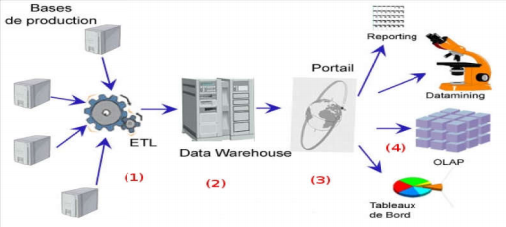
\includegraphics[width=95mm]{src_img/fonctionnementOLAP.png}
  \caption{Fonctionnement OLAP \supercite{fonctionnementSOLAP}}
  \label{fig:olap}
\end{figure}
\paragraph{}Comme indiqué précédemment, les données NoSQL sont hétérogènes et c’est particulièrement le cas avec les données géographiques qui comprennent des données géométriques (lignes, points, polygones) mais également des données associées. Cette structure amène des besoins d’analyse\cite{solap} plus approfondies.

\begin{table}[h!]
    \centering
	\begin{tabular}{|p{5cm}|p{7cm}|} 
  	\hline
  	\textbf{Critère} & \textbf{Valeur} \\
  	\hline
  	1.1 : respect principes Codd & Oui, il respecte les relations \\
  	\hline
  	1.2 : schéma utilisé & Fixe \\
  	\hline
  	1.3 : modèle & Relationnel \\
  	\hline
  	1.4 : langage de requêtage & SQL avec quelques autres fonctions (ROLLUP, GROUPING, etc)  \\
  	\hline
	\end{tabular}
    \caption{Table des critères concernant SOLAP}
    \label{tab:critere-solap}
\end{table}

\section{Les SIG as a Service, une offre en expansion}
\paragraph{}Depuis quelques années, le cloud computing avec ses paradigmes s'est imposé dans la distribution de logiciels et a permis à de nouvelles plateformes de se développer. Les entreprises développant les SIG ont donc dû s'adapter pour proposer des architectures plus flexibles et simples d'utilisation.

\paragraph{}L'augmentation des plateformes géospatiales dans le cloud a entraîné un changement de comportement vis-à-vis du travail des données spatiales. Parmi les principaux avantages, il y a le partage d'informations facilité, la spécialisation de certains outils, la simplicité obtenue dans l'utilisation, la baisse des coûts et le potentiel de croissance.

\paragraph{}Le Software as a Service (SaaS) permet aux utilisateurs d'utiliser une solution installée sur des serveurs distants et non sur la machine de ce dernier. Cela passe essentiellement par un service en ligne avec abonnement. Parmi les SIG qui utilisent le SaaS, nous avons ArcGIS, développé par ESRI. Cet outil permet le reporting et la création de tableaux de bord métier à partir de cartographie et d'analyse spatiale. D'autres outils comme CARTO, déjà cité auparavant et MapBox, fournisseur de cartes personnalisées utilisent également cette architecture.

\paragraph{}Une autre catégorie de plateformes est le PaaS, le Platform as a Service, où le fournisseur cloud maintient l'infrastructure et le matériel et le client maintient pour sa part l'application. ArcGis founit aussi cet architecture en terme de solution tout comme les API de Google Maps ou Geocode Dataflow de Microsoft.

\paragraph{}Le DaaS, Data as a Service, est le dernier type d'architecture utilisé dans les SIG. Il permet à l'utilisateur d'être uniquement facturé par le fournisseur pour les données qu'il souhaite utiliser. Cela passe par la délégation du stockage et de la gestion des données. Cela est par exemple utilisé par les outils de cartographie comme Google Maps ou OpenStreetMap.


\section{Synthèse et critique}

Nous avons pu dans cette partie comparer l'exemple en terme de gestion des SIG. D'un côté, PostGIS utilise les fonctions traditionnelles des SGBD relationnels pour gérer les objets géométriques. Il se base sur de nombreux standards à la fois ISO et OGC pour permettre une meilleure interopérabilité. De l'autre, nous avons MongoDB qui grâce à sa gestion des documents permet une gestion optimisée des documents comme l'est le GeoJSON. Egalement, face aux besoins de plus en plus importants d'analyses multidimensionnelles, SOLAP permet d'intégrer la dimension spatiale aux outils traditionnels. Le développement du cloud computing a également apporté diverses possibilités.

\paragraph{}De petits projets utilisant des données géographiques peuvent utiliser des systèmes de gestion de données relationnels comme PostGreSQL et son module PostGIS. Cependant, avec l'accroissement continu de la quantité de données échangées dans le monde, dont 80\% représentent des données spatiales, il s'avère plus qu'important d'utiliser des architectures de bases de données adéquates et les bases de données telles que MongoDB peuvent représenter une solution. Si une analyse multidimensionnelle est nécessaire, il est également possible de se tourner vers SOLAP.

\chapter{Application}
\section{La proposition}
\subsection{L'objectif}
\paragraph{}Le but de l'application qui va suivre est de comparer différents modèles à la fois NoSQL et relationnels dans le but de déterminer le plus adapté par rapport aux données géographiques des SIG. Différents tests seront réalisés afin de mettre en lumière les forces et faiblesses de chacun. Lequel est le plus simple à modéliser, lequel a les meilleures vitesses d'exécution, lequel facilite la représentation sont des questions qui pourront se poser.


\subsection{Le choix des modèles}
\paragraph{}Afin de répondre à la question générale, plusieurs SGBD et modèles seront utilisés. Le premier sera le document. Son principal avantage est celui d'unité de la structure, supprimant le besoin de réaliser des jointures et permettant une meilleure adaptation à la distribution. Ce modèle s'avère grandement utilisé dans les outils de cartographie actuels comme avec le \newacronym{GML}{GML}{Geography Markup Language} \acrshort{GML} et ses dérivés : le \newacronym{KML}{KML}{Keyhole Markup Language} \acrshort{KML} utilisé par Google Earth et le OSM XML utilisé par OpenStreetMap. La structure des grammaires, encadrées par l'\acrfull{OGC} permet une meilleure interopérabilité.
%Le premier modèle qui sera utilisé sera le modèle graphe. Sa structure avec des noeuds et des arcs s'avère l'une des plus adaptées dans le cadre par exemple de calculs de distances.
%PARAGRAPHE A MODIFIER

%\paragraph{}Par ailleurs, un autre modèle sera implémenté, ce 

\paragraph{}Afin de comparer les modèles NoSQL à des modèles plus traditionnels que sont les bases de données relationnels, une étude sera faite sur une base qui suit les principes de Codd avec relations et nuplets.

\subsection{Le jeu d'essai}
\paragraph{}Le jeu d'essai utilisé dans le cadre de ce mémoire correspond aux résultats des élections municipales de 2020, plus précisément de son premier tour. Les données sont issues des sources gouvernementales fournies par le Ministère de l'Intérieur sur \url{data.gouv.fr}.

\paragraph{}Le fichier initial comprenait 68 815 lignes de données qui représentaient chacune les résultats d'un bureau de vote dans toutes les communes des 103 départements français (Outre-mer compris). Cependant, au vue de la quantité trop importante de données, il a été choisi de prendre uniquement les résultats franciliens (d'Ile-de-France) qui limite donc les données à 7 326 bureaux de votes, répartis sur 1268 communes à travers 8 départements. 

\paragraph{}Parmi les données répertoriées dans le fichier, nous avons les informations sur le département et la commune avec pour chacun leur nom et leur code. Sont également présentes les données sur le bureau de code : son numéro, le nombre d'inscrits, le nombre de votants, d'abstention, du nuls ou de blancs avec différents pourcentages basés sur le nombre de votants ou d'inscrits. Après cela, il y a les données sur les listes avec un numéro, la nuance politique et les informations sur le candidat (nom, prénom et sexe). Aussi, selon si c'est une commmune avec candidature par liste ou candidat, le nom de la liste est renseigné ou non. Concernant les résultats, sur chaque ligne de bureau de vote et pour chaque liste ou candidat, il y a le nombre de voix et le pourcentage par rapport au nombre d'inscrits et de votants.

\paragraph{}Par rapport à ce fichier, il a également été choisi de faire un tri comme un certain nombre de données calculées sont présentes alors qu'elles peuvent être calculées par le SGBD.

%Le fichier comprend 68 815 lignes de données quants i présentent chacune les résultats de chaque bureau de vote dans toutes les communes dans tous les départements de France métropolitaine et d'Outre-mer. Parmi les informations présentées, nous avons :
%\begin{itemize}
    %\item les informations sur le département : le code et le nom
    %\item les informations sur la commune : la partie commune du code INSEE et le nom
   % \item le bureau de vote : son code, le nombre d'inscrits, de votants, d'abstention et leur pourcentage respectif ainsi que le nombre de bulletins nuls, blancs et exprimés et leur pourcentage par rapport au nombre de votants et d'inscrits
    %\item les informations sur les listes : un code, le nuance politique, le sexe, le nom et prénom de la tête de liste et le nom de la liste associée
    %\item les résultats de chaque liste : le nombre de voix obtenues et le pourcentage par rapport au nombre de votants et d'inscrits
%\end{itemize}

%\paragraph{}Cependant, après réflexions autour de la pertinence de certaines données, il a été choisi d'enlever les pourcentages car même si ils évitent de devoir effectuer des calculs, ils occupent un espace qui pourrait être libéré.
%couplées aux données territoriales pour faire correspondre communes, départements, régions

\subsection{Les outils utilisés}
\paragraph{}Plusieurs outils seront utilisés dans le cadre de la réalisation de cette application. Plusieurs SGBD seront utilisés :
\begin{itemize}
    \item MySQL comme base de données relationnelle
    \item BaseX pour les aspects document
    %\item OrientDB ou Neo4j pour les graphes
\end{itemize}

\section{L'utilisation d'un modèle relationnel}

\subsection{Modélisation et implémentation}
\paragraph{}Le \acrshort{MCD} ci-dessous correspond à la représentation la plus adaptée du jeu de données en y enlevant les données calculées. On peut y voir qu'un département est composé de plusieurs communes avec pour chacune des bureaux de vote, des candidats et listes. La relation bureau de vote-candidat permet d'obtenir le nombre de voix obtenu pour ce candidat dans ce bureau.


%Le modèle conceptuel de données ci-dessous correspond à la représentation la plus adaptée des données. A partir de ce dernier a été généré un script SQL permettant la création de la base de données.
%\paragraph{}Dans le \acrshort{MCD} ci-dessous, on peut y voir qu'un département est composé de plusieurs communes et dépendent de ce département. Il peut par exemple avoir plusieurs villes avec le même nom mais dans des départements différents. Pour chacune de ces villes, il y a des bureaux de votes et des candidats ou listes qui lui sont associés et ces derniers obtiennent des résultats aux élections.
%Il prend en compte un certain tri des données. En effet, de nombreuses données calculées, des pourcentages, étaient présents. Cependant, ces données occupent de l'espace inutilement sachant que ces calculs peuvent être effectués par le SGBD.
\begin{figure}[!htp]
  \centering
  \includegraphics[width=.9\textwidth]{./src_img/image_mcd.png}
  \caption{Modèle Conceptuel de données}
  \label{fig:mcd}
\end{figure}

\subsection{Le peuplement de la base}


\paragraph{}Avec le MCD, un script SQL a permis la création de la base de données puis, pour la compléter, un code similaire à ce pseudo-code a été utilisé :\newline
\begin{algorithm}[H]
\KwData{fichier CSV}
 \KwResult{Base de données remplie}
 initialisation fichier\;
 \While{toutes les lignes ne sont pas parcourues}{
 \If{departement non présent}{ajouter département dans la base}
  \If{commune non présente}{ ajouter commune dans la base}
 \If{bureau de vote non présent}{ ajouter bureau dans la base}
 \While{ligne de données non finie d'être parcourue}{
 \If{liste/candidat non présent}{ ajouter liste/candidat dans la base}
 ajouter résultat\;
 }
 }
 \caption{Algorithme de peuplement de la base}
\end{algorithm}
\paragraph{}Dans cet algorithme, pour chaque élément qu'on souhaite ajouter, une vérification est nécessaire afin d'éviter d'avoir des doublons de bureaux ou candidats dans la base.

\paragraph{}En partant des critères définis au début de l'état de l'art, nous allons donc évaluer cette base de données.
\begin{table}[h!]
    \centering
	\begin{tabular}{|p{5cm}|p{7cm}|} 
  	\hline
  	\textbf{Critère} & \textbf{Valeur} \\
  	\hline
  	2.1 : taille occupé & 5,87 Mo \\
  	\hline
  	2.2 : nombre d'objets & 64 873 \\
  	\hline
	\end{tabular}
    \caption{Table des critères concernant la base de données MySQL}
    \label{tab:critere-mysqlbase}
\end{table}
\subsection{L'interrogation d'un SGBD relationnel}
\paragraph{}Afin de vérifier des performances de la base de données, diverses requêtes vont être réalisées :
\subsubsection{Une requête de recherche}
\paragraph{}La première requête va lister les communes des Yvelines (78) comprenant un 'r' dans leur nom avec le nombre de votants respectifs, triés par ordre décroissant.
%\paragraph{}Cette première requête va rechercher la liste des communes et leurs nombres de votants par ordre décroissant pour celles situées dans les Yvelines (78) et comprenant un R dans leur nom.
\paragraph{}Cette requête retourne 162 villes parmi lesquelles Versailles et Saint-Germain-en-Laye. Elle a été réalisée en 5 ms et a manipulé 814 objets (villes et bureaux de vote).

\iffalse
\begin{figure}[!ht]
    \begin{verbatim}
SELECT nom_ville, SUM(nb_inscrits) as nb_insc 
FROM ville, bureau_vote 
WHERE ville.code_dep = bureau_vote.code_dep 
  AND ville.code_ville = bureau_vote.code_ville 
  AND nom_ville LIKE '%r%' AND ville.code_dep='78' 
GROUP BY nom_ville 
ORDER BY nb_insc desc;
\end{verbatim}
    \caption{Requête de recherche}
\end{figure}
\fi

\subsubsection{Une requête de calcul et regroupement}
\paragraph{}La deuxième requête est destinée à calculer pour chaque département francilien le nombre de communes ayant un vote par liste et le nombre de celles ayant un vote par poste. Voici donc le résultat qu'elle a permis d'obtenir :
\begin{figure}[!htp]
  \centering
  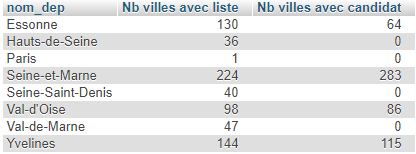
\includegraphics[width=0.6\textwidth]{./src_img/req2_sql.png}
  \caption{Données extraites de la 2ème requête}
  \label{fig:req2}
\end{figure}
\paragraph{}Cette requête, réalisée en 126 millisecondes en touchant à 12 574 objets, avait une petite spécificité. Habituellement, pour déterminer si l'élection est par liste ou candidat, on se base sur la population mais le jeu de données ne comporte pas cette donnée. Nous nous basons donc sur le champ du nom de la liste, vide si c'est une élection par candidat. %Habituellement, pour savoir si une ville a une élection par liste ou candidat, on se base sur la population de celle-ci. Hors, dans le jeu de données, nous n'avons que le nombre d'inscrits sur les listes électorales, excluant donc les mineurs. Pour savoir le type de l'élection, il a donc été choisi de vérifier si le champ du nom de liste parmi les listes et candidats présents étaient remplis ou non.
%\paragraph{}La deuxième requête est destinée à calculer pour chaque département francilien le nombre de communes ayant un vote par liste ou un vote par candidat. \newline Pour définir le type du vote, il est habituellement réalisé en fonction du nombre d'habitants de la commune. Or, ici, nous n'avons que le nombre d'inscrits sur les listes électorales, ce qui exclut donc les mineurs. Pour déterminer si le vote dans une commune se fait par liste ou candidat, nous nous sommes basés sur le nom de liste, vide si c'est une élection par candidat.
\iffalse
\begin{figure}[!ht]
    \begin{verbatim}
SELECT nom_dep, 
(SELECT count(distinct(nom_ville)) as nb from ville, liste
  where liste.code_dep=ville.code_dep and
  ville.code_ville=liste.code_ville  and
  liste.code_dep=dep.code_dep and 
  length(nom_liste)<>0) as `Nb villes avec liste`, 
(SELECT count(distinct(nom_ville)) as nb from ville, liste
  where liste.code_dep=ville.code_dep and
  ville.code_ville=liste.code_ville and
  liste.code_dep=dep.code_dep and 
  length(nom_liste)=0) as `Nb villes avec candidat`
FROM departement dep
GROUP BY nom_dep;
\end{verbatim}
    \caption{Requête de calcul et regroupement}
\end{figure}
\fi

%\paragraph{}Cette requête a été réalisée en 126 millisecondes.

%nombre moyen de listes par région

\subsubsection{Des taux en fonction de différents critères}
\paragraph{}Il a également choisi de vérifier les fonctions de calcul. Deux requêtes ont donc été réalisées dans ce but. La première liste les communes d'Ile-de-France triées suivant une absention décroissante. Elle a retournée 1268 résultats (soit toutes les communes franciliennes) en 4,96 ms tout en lisant 8 594 objets.
%- les régions/communes ayant enregistré le plus grand taux d'abstention

\iffalse
SELECT nom_ville, ville.code_dep,  ((SUM(nb_abstention)/SUM(nb_inscrits))*100) as taux FROM ville, bureau_vote WHERE ville.code_dep=bureau_vote.code_dep AND ville.code_ville=bureau_vote.code_ville GROUP BY nom_ville ORDER BY taux desc
\fi
%temps : 4,96 ms
\paragraph{}La deuxième requête retourne le taux de participation par département. Elle retourne donc 8 objets en 1,74 millisecondes tout en touchant à 8 602 objets.
%- taux de participation par région/commune
\iffalse
SELECT departement.nom_dep, SUM(nb_inscrits) as nbinsc, SUM(nb_votants) as nbvot, ((SUM(nb_votants)/SUM(nb_inscrits))*100) as taux
FROM departement, ville, bureau_vote WHERE departement.code_dep=ville.code_dep AND ville.code_dep=bureau_vote.code_dep AND ville.code_ville=bureau_vote.code_ville
GROUP BY departement.nom_dep
ORDER BY taux desc
\fi
%temps : 1,74 ms
\subsubsection{Une requête de mise à jour}
\paragraph{}La dernière requête est une mise à jour. Il a été choisi de modifier le nom d'une liste d'une commune. La requête a été réalisée en 0, 00044 ms en lisant qu'un seul objet.

%temps : 0,00044 ms
\subsubsection{Synthèse des résultats}
\paragraph{}La table \ref{tab:critere-req1mysqlbase} représente les résultats des critères définis auparavant. On peut y apercevoir une durée inférieure à 5 ms pour la plupart des requêtes mais également, en parallèle, un grand nombre d'objets manipulés.
\begin{table}[!h]
    \centering
	\begin{tabular}{|p{3cm}|p{3cm}|p{3cm}|p{3cm}|} 
  	\hline
  	\textbf{Requête} & \textbf{3.1 : temps} & \textbf{3.2 : nombre de résultats} & \textbf{3.3 : objets manipulés} \\

  	\hline
  	Requête 1 & 5 ms & 162 & 814 \\
  	\hline
    Requête 2 & 126 ms & 8 & 12 574 \\
    \hline
    Requête 3 & 4,96 ms & 1268 & 8 594 \\
    \hline
    Requête 4 & 1,74 ms & 8 & 8 602 \\
    \hline
    Requête 5 & 0,00044 ms & & 1 \\
    \hline
	\end{tabular}
    \caption{Table des critères concernant les requêtes via MySQL}
    \label{tab:critere-req1mysqlbase}
\end{table}
\newpage
\subsection{La représentation des données depuis MySQL}
\paragraph{}Après avoir pu comparer les résultats des requêtes, il peut être également intéressant de faire le tour des solutions possibles de représentation des données, MySQL ne permettant pas la visualisation graphique. Il existe deux catégories.

\subsubsection{Les logiciels de datavisualisation}
\paragraph{}Un grand nombre d'outils permettent de visualiser des données, répartis entre ceux uniquement dédiés à la visualisation et ceux permettant à l'aide à la décision via de la BI (Business Intelligence). Parmi ces outils, nous avons Tableau Software, Qlik Sense, Power BI et SAP Business Object BI. Ces outils permettent à la fois la représentation sous forme d'histogramme, de diagramme circulaire, de treemap voire même de cartes.
\subsubsection{Les librairies}
\paragraph{}En plus de ces logiciels, des librairies existent pour fonctionner avec diverses technologies pour les utiliser au sein de projets. Des langages orientés objet tels que Java, C\# peuvent les utiliser tout comme PHP, Ruby, Python ou JavaScript. Parmi ces librairies qui permettent la visualisation de graphiques, nous avons Chart.js, D3.js, Google Chart API ou Highcharts.

\paragraph{}La figure \ref{fig:graphMySQL} est par exemple le résultat de la requête concernant l'abstention par région. Ce diagramme a été réalisé grâce à Chart.js.

\begin{figure}[!htp]
  \centering
  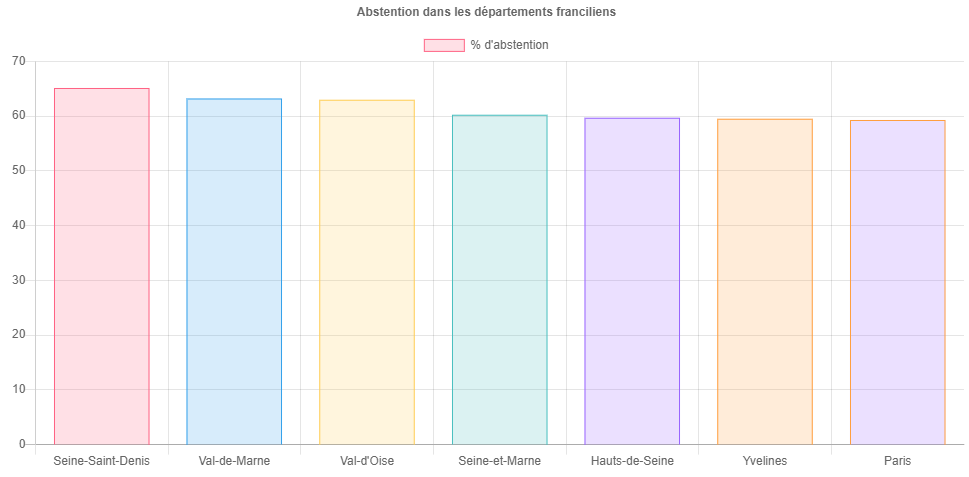
\includegraphics[width=0.6\textwidth]{./src_img/chartMySQLData.png}
  \caption{Graphique utilisant les données MYSQL}
  \label{fig:graphMySQL}
\end{figure}

%des requêtes, pour quoi ne chercher côté visualisation maintenant? 
%Est-ce que BaseX a des outils de visualisation intégrés?
%visualisation tableau des résultats des requêtes, mais de la visualisation graphique! Je ne connais pas BaseX pour te suggérer une piste, mais je pense qu'il est très intéressant de comparer  la possibilité d'affichage graphique des données relationnelles et données en documents (en brut ou résultat d'un requête).


\section{L'utilisation d'un modèle orienté document}

\subsection{Modélisation}
\paragraph{}La modélisation pour avoir un document s'est également basé sur une réflexion autour des données présentes. Celles présentes et répétées de nombreuses fois telles que les départements et communes ont été priorisées. Pour la gestion des bureaux et des listes, il a été choisi de proriser les bureaux de vote car ils correspondaient à la caractéristique principale de chaque ligne du jeu d'essai.

\begin{figure}[!htp]
  \centering
  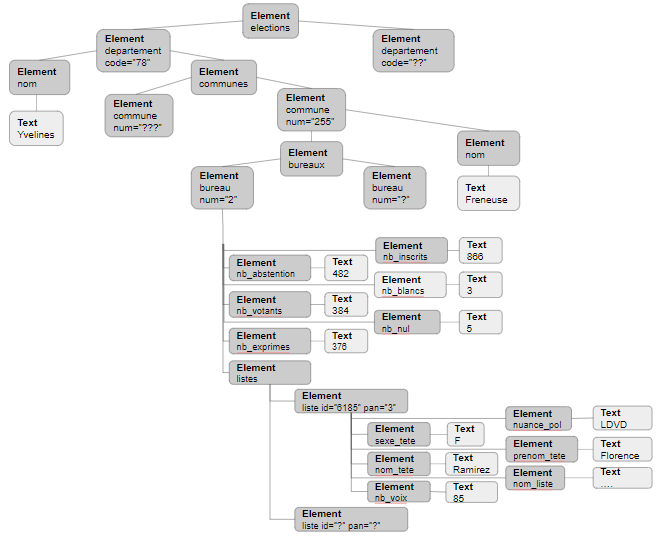
\includegraphics[width=\textwidth]{./src_img/structure_document.png}
  \caption{Modèle document}
  \label{fig:model_doc}
\end{figure}

\paragraph{}De la réflexion présentée est issue le modèle ci-dessus (figure \ref{fig:model_doc}) où nous avons à la base de la structure les départements dans lesquels sont ajoutés les communes qui le composent. Dans chacune de ces villes, nous retrouvons les différents bureaux de votes avec pour chacun les listes présentes, leurs informations et les résultats récoltés.
%\begin{figure}[!htb]
   %\begin{minipage}{0.48\textwidth}
    % \centering
     %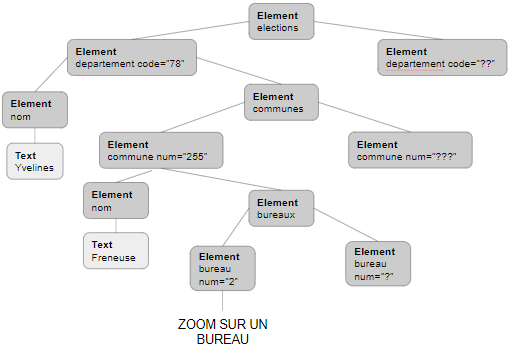
\includegraphics[width=\linewidth]{./src_img/modele_doc1.png}
     %\caption{Partie haute (département, ville et bureau)}\label{Fig:modele_doc1}
   %\end{minipage}\hfill
   %\begin{minipage}{0.48\textwidth}
   %  \centering
    % 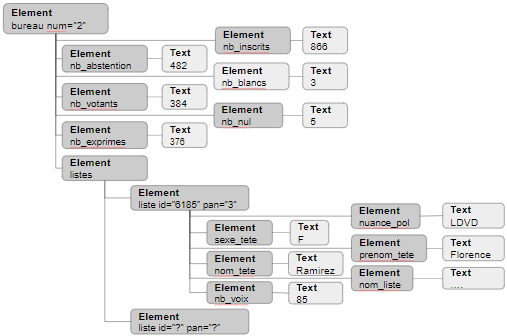
\includegraphics[width=\linewidth]{./src_img/modele_doc2.png}
    % \caption{Partie basse (détail d'un bureau et des listes et résultats)}\label{Fig:modele_doc2}
   %\end{minipage}
%\end{figure}

\subsection{L'implémentation du modèle avec les données}
\paragraph{}L'implémentation s'est faite à partir de ce modèle afin de donner un document XML apte à être utilisé. Par la suite, les données ont pu être insérées suivant l'algorithme suivant.

%a modifier
\begin{algorithm}[H]
 \KwData{fichier CSV}
 \KwResult{Base de données remplie}
 initialisation fichier\;
 \While{toutes les lignes ne sont pas parcourues}{
 \If{departement non présent}{ajouter département dans la base}
 déplacement dans le noeud du département\;
  \If{commune non présente}{ ajouter commune dans la base}
 déplacement dans le noeud de la commune\;
 \If{bureau de vote non présent}{ ajouter bureau dans la base}
 déplacement dans le noeud du bureau\;
 \While{tous les candidats/listes ne sont pas traités}{
 ajouter liste/candidat dans la base\;
 ajouter le résultat associé\;
 }
 }
 \caption{Algorithme de peuplement de la base}
\end{algorithm}

\paragraph{}En partant des critères définis au début de l'état de l'art, nous allons donc évaluer cette base de données.
\begin{table}[h!]
    \centering
	\begin{tabular}{|p{3cm}|p{9cm}|} 
  	\hline
  	\textbf{Critère} & \textbf{Valeur} \\
  	\hline
  	2.1 : taille & 10,58 Mo \\
  	\hline
  	2.2 : nombre d'objets & 673 942 noeuds parmi lesquels 53 575 correspondent aux départements, villes, bureaux et listes \\
  	\hline
	\end{tabular}
    \caption{Table des critères concernant la base de données XML}
    \label{tab:critere-xmlbase}
\end{table}
\paragraph{}Les résultats obtenus sont cohérents avec la structure du fichier XML, plus robuste qu'une base de données SQL.
\iffalse
\begin{figure}[!htb]
   \begin{minipage}{0.48\textwidth}
     \centering
     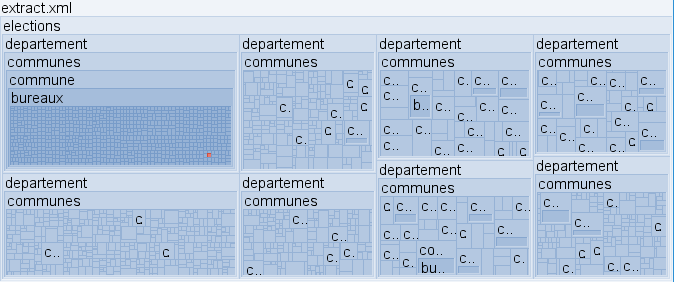
\includegraphics[width=.9\linewidth]{./src_img/modelisation_doc_1.png}
     \caption{Aperçu global}\label{Fig:doc_global}
   \end{minipage}\hfill
   \begin{minipage}{0.48\textwidth}
     \centering
     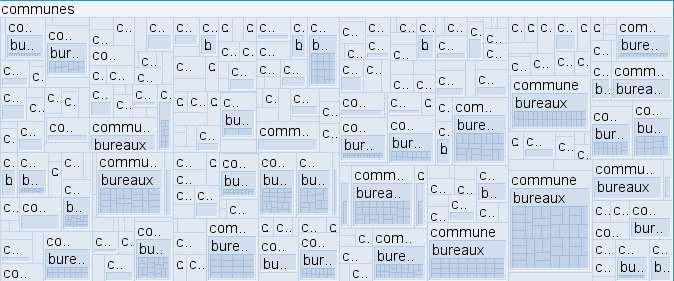
\includegraphics[width=.9\linewidth]{./src_img/modelisation_doc_2.png}
     \caption{Zoom sur les communes d'un département}\label{Fig:doc_dep}
   \end{minipage}
      \begin{minipage}{0.48\textwidth}
     \centering
     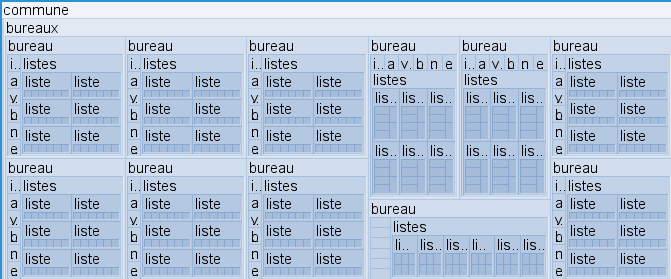
\includegraphics[width=.9\linewidth]{./src_img/modelisation_doc_3.png}
     \caption{Zoom sur une commune}\label{Fig:doc_commune}
   \end{minipage}\hfill
   \begin{minipage}{0.48\textwidth}
     \centering
     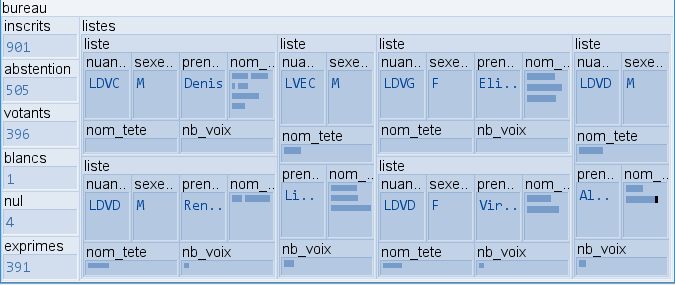
\includegraphics[width=.9\linewidth]{./src_img/modelisation_doc_4.png}
     \caption{Zoom sur un bureau}\label{Fig:doc_bureau}
   \end{minipage}
\end{figure}
\fi

\subsection{L'interrogation d'un SGBD document}


\paragraph{}Afin de vérifier des performances de la base de données, nous allons reprendre les mêmes besoins que pour le SGBD relationnel :

\subsubsection{Une requête de recherche}
\paragraph{}Nous reprenons la requête qui va lister les communes des Yvelines (78) comprenant un 'r' dans leur nom avec le nombre de votants respectifs, triés par ordre décroissant.
%\paragraph{}Cette première requête va rechercher la liste des communes et leurs nombres de votants par ordre décroissant pour celles situées dans les Yvelines (78) et comprenant un R dans leur nom.
\paragraph{}Cette requête retourne 162 villes parmi lesquelles Versailles et Saint-Germain-en-Laye. Elle a été réalisée en 11,15 ms et a manipulé 1 630 objets du noeud initial au noeud du nombre de votants.


\iffalse
2 + 162 communes à R + 162 bureaux + 652 + 652 = 1630
\begin{figure}[!ht]
    \begin{verbatim}
for $x in //elections/departement[@code="78"]/communes/
commune[contains(nom,'r')]
 let $nom := $x/nom
 let $somme := sum($x/bureaux/bureau/inscrits)
 order by xs:integer($somme) descending
return <RESULT> {$nom} - {$somme} </RESULT>

\end{verbatim}
    \caption{Requête de recherche}
\end{figure}
\fi
%\paragraph{}Cette requête possède 162 résultats y compris Versailles ou Saint-Germain-en-Laye et a été réalisé en 15,62 millisecondes.



\subsubsection{Une requête de calcul et regroupement}
\paragraph{}La deuxième requête est destinée à calculer pour chaque département francilien le nombre de communes ayant un vote par liste et le nombre de celles ayant un vote par poste. 

\paragraph{}Cette requête, réalisée en 23,56 millisecondes en touchant à 2 553 objets, avait une petite spécificité. Comme énoncé auparavant, on distingue des candidats seuls aux listes par le nom de liste, vide si c'est une élection par candidat. Cependant, pour éviter de devoir répéter les opérations sur chaque liste sur chaque bureau de vote, il a été choisi de vérifier une seule liste d'un seul bureau.

\iffalse
\begin{figure}[!ht]
    \begin{verbatim}
for $x in //elections/departement
 let $nom := $x/nom
 let $commune := $x/communes/commune
 let $nbListe := count($commune[bureaux/bureau[1]/
 listes/liste[1]/nom_liste])
 let $nbCandidat := count($commune[bureaux/bureau[1]/
 listes/liste[1]/not(nom_liste)])
return <RESULT> {$nom} - {$nbListe} - {$nbCandidat} </RESULT>
\end{verbatim}
    \caption{Requête de calcul et regroupement}
\end{figure}
\fi
%\paragraph{}Le résultat obtenu est bien la liste des départements avec pour chacun le nombre de communes avec liste et le nombre de celles avec candidats. La requête a été faite en 84.66 millisecondes.

\subsubsection{Des taux en fonction de différents critères}
\paragraph{}Il a également choisi de vérifier les fonctions de calcul. Deux requêtes ont donc été réalisées dans ce but.

\paragraph{}La première liste les communes d'Ile-de-France triées suivant une absention décroissante. Elle a retournée 1268 résultats (soit toutes les communes franciliennes) en 74 ms tout en lisant 17 205 objets.
%temps : 4,96 ms

\iffalse
for $x in //elections/departement/communes/commune
 let $nom := $x/nom
 let $inscrits := number(sum($x/bureaux/bureau/inscrits))
 let $abs := number(sum($x/bureaux/bureau/abstention))
 let $pct := $abs div $inscrits * 100
  order by xs:integer($pct) descending
return <RESULT> {$nom} - {$inscrits} - {$abs} - {$pct}</RESULT>
\fi
%temps : 91ms / 74,4


\paragraph{}La deuxième requête retourne le taux de participation par département. Elle retourne donc 8 objets en 43 millisecondes tout en touchant au même nombre d'objets.

\iffalse
for $x in //elections/departement
 let $nom := $x/nom
 let $insc := sum($x/communes/commune/bureaux/bureau/inscrits)
 let $vot := sum($x/communes/commune/bureaux/bureau/votants)
 let $pct := $vot div $insc * 100
return <RESULT> {$nom} - {$pct}</RESULT>
\fi
%temps 63 ms / 43

\subsubsection{Une requête de mise à jour}
\paragraph{}La dernière requête est une mise à jour, celle du prénom de la tête de liste dans une commune à trois bureaux de vote. La requête a été réalisée en 3,45 ms en lisant 13 noeuds dont 3 à modifier.

%temps : 0,00044 ms
\subsubsection{Synthèse des résultats}
\paragraph{}La table \ref{tab:critere-req1docbase} représente les résultats des critères définis auparavant. On peut y apercevoir une durée comprise entre 3 et 74 ms pour la plupart des requêtes mais également, en parallèle, un grand nombre d'objets manipulés, plus important que pour une base de données relationnelle. Nous pouvons également noté que sur la requête 2, BaseX donne un résultat beaucoup plus rapide que MySQL.
\begin{table}[h!]
    \centering
	\begin{tabular}{|p{3cm}|p{3cm}|p{3cm}|p{3cm}|} 
  	\hline
  	\textbf{Requête} & \textbf{3.1 : temps} & \textbf{3.2 : nombre de résultats} & \textbf{3.3 : objets manipulés} \\

  	\hline
  	Requête 1 & 11,15 ms & 162 & 1 630 \\
  	\hline
    Requête 2 & 23,56 ms & 8 & 2 553 \\
    \hline
    Requête 3 & 74 ms & 1 268 & 17 205 \\
    \hline
    Requête 4 & 43 ms & 8 & 17 205 \\
    \hline
    Requête 5 & 3,45 ms & & 13 \\
    \hline
	\end{tabular}
    \caption{Table des critères concernant les requêtes via BaseX}
    \label{tab:critere-req1docbase}
\end{table}

\subsection{La représentation des données depuis un document}
\paragraph{}Tout comme le modèle relationnel, il est intéressant de voir comment les données peuvent être représentées. Nous allons voir ici le cas du jeu de données testé mais également les possibilités fournies avec les outils manipulant des données stockées sous forme de document.


\subsubsection{La visualisation au sein de BaseX}
\paragraph{}BaseX propose plusieurs types de visualisations au sein de son outil dont des treemap, des graphiques entre autres. En voici un exemple pour un bureau avec le treemap correspondant (figure \ref{Fig:treemapbureau}) et le graphique associé montant le nombre de voix obtenues par chaque liste (figure \ref{Fig:graphebureau}).
\begin{figure}[!htb]
   \begin{minipage}{0.48\textwidth}
     \centering
     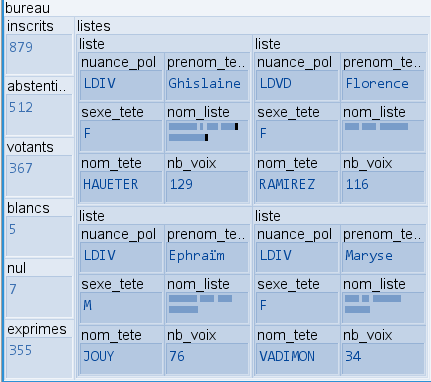
\includegraphics[width=.6\linewidth]{./src_img/contenubureau.png}
     \caption{TreeMap d'un bureau}\label{Fig:treemapbureau}
   \end{minipage}\hfill
   \begin{minipage}{0.48\textwidth}
     \centering
     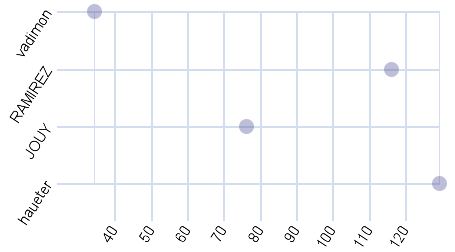
\includegraphics[width=.7\linewidth]{./src_img/graphbureau.png}
     \caption{Graphique du même bureau}\label{Fig:graphebureau}
   \end{minipage}
\end{figure}
\paragraph{}La critique qui peut être faite à BaseX est la limitation qu'elle possède au niveau des graphiques. Elle peut afficher les correspondances de plusieurs données liées aux différents objets mais ne peut traiter de requêtes. Il est donc intéressant de voir les autres possibilités.

\subsubsection{Les possibilités fournies par les outils gérant des documents}
\paragraph{}Pour le traitement de données géographiques, il peut être intéressant de réaliser des visualisations sous forme de cartes. Cependant, le jeu de données utilisé ne comprend pas les caractéristiques permettant d'en réaliser. En effet, pour avoir une représentation géographique, il est nécessaire d'avoir les coordonnées, c'est-à-dire la latitude et la longitude. Si ces données étaient présentes, des formats tels que le \acrfull{GML} ou le \acrfull{KML} auraient pu être utilisés pour afficher les informations par exemple sur Google Earth avec les données sous format \acrshort{KML}.

\paragraph{}Ces dernières années, le \newacronym{JSON}{JSON}{JavaScript Object Notation}\acrshort{JSON} est devenu de plus en plus utilisé, devenant donc une référence dans le traitement de données. Bien que moins sécurisé et non produit par l'\acrshort{OGC}, il se révèle plus léger et plus lisible que le XML \cite{xmljsoncomparison}. De nombreux outils tels que MongoDB sont familiers avec ce langage. Son dérivé, le GeoJSON s'est imposé dans le traitement de données géographiques \cite{geojsonxml}. Avec sa base venant du JavaScript, il permet une adaptation simple avec les nombreuses librairies de visualisation de données déjà présentées, Leaflet2 utilisée notamment par OpenStreetMap mais également D3.js.


\chapter{Synthèse et discussion}

\paragraph{}Ma proposition a été de comparer deux bases de données, une relationnelle, une NoSQL, sur leurs aspects techniques et leurs performances. Parti d'une même source, j'ai souhaité vérifier que la comparaison donnait l'avantage aux bases de données NoSQL. Pour ce faire, un retour sur chaque étape sera fait.

\paragraph{}Tout d'abord, la modélisation côté relationnel possède certains avantages. En effet, un formalisme, assez simple d'apprentissage, via Merise et le \newacronym{MCD}{MCD}{modèle conceptuel de données} \acrfull{MCD}, permet d'organiser les données de façon optimale. Nous ne retrouvons pas cette méthodologie côté document. Par ailleurs, la réflexion est plus importante côté relationnel afin de gérer les contraintes. De ce fait, j'attribue comme note au relationnel un 7/10 et un 5 au modèle document.

%Tout d'abord, vis-à-vis de la modélisation, le relationnel possède certains avantages. Il possède un formalisme, assez simple d'apprentissage qui permet de modéliser les données. Un \newacronym{MCD}{MCD}{modèle conceptuel de données} \acrfull{MCD} permet de préparer de manière optimale la base de données. A l'inverse, aucun formalisme est présent et commun aux modèles NoSQL, la modélisation est donc rendue plus compliquée et comme il est visible dans la figure \ref{fig:model_doc}, elle nécessite l'affichage des données. Cependant, vis-à-vis des données présentes dans le jeu initiale, la réflexion a été plus importante pour le modèle relationnel avec les contraintes à gérer. Si je dois attribuer une note, la modélisation relationnelle obtient un 7/10 et celle document un 5.

%\paragraph{}La deuxième étape est l'implémentation, elle comprend à la fois la réalisation de la structure physique et l'ajout des données. Les procédures ont été assez similaires pour le remplissage des départements, villes et bureaux avec une vérification de la présence ou non à chaque itération des données. Par la suite, l'ajout des listes et de leurs résultats a nécessité plus de vérifications côté relationnel. Cela au fait que le modèle document a uniquement besoin de reporter les données au bon endroit alors que le traitement côté relationnel doit vérifier la cohérence vis-à-vis des listes et du bureau. De ce fait, j'attribue un 6 côté document et un 4 côté relationnel.

\paragraph{}La deuxième étape est l'implémentation qui se divise en deux étapes : la création de la structure qui se réalise assez simplement des deux côtés et l'ajout des données qui possède quelques spécificités. Pour les départements, villes et bureaux de vote, le processus est assez simple. J'attribue un 4 au modèle relationnel dû aux vérifications supplémentaires nécessaires pour ajouter candidats et résultats. Ne nécessitant pas cette étape, le modèle document obtient un 7.


%C'est à l'ajout des listes ou candidats et de leurs résultats que cela diffère. En effet, côté document, les données ont uniquement besoin d'être reportées au bon endroit et les champs vides n'ont pas à être créés, c'est le cas par exemple du nom de liste, absent chez les candidats seuls. Du côté relationnel, il est nécessaire de vérifier la cohérence, de vérifier si la liste est déjà créée ou non pour éviter les erreurs à l'ajout. Egalement, le champ concernant le nom de liste peut se retrouver vide. 

\paragraph{}Pour l'interrogation, au vu de ce qui a été obtenu, il s'avèrent que les deux modèles obtiennent des résultats tout à fait convenables avec des traitements durant moins d'une seconde. Cependant, il est possible de voir que le relationnel a répondu aux requêtes un peu plus rapidement. Cela peut s'expliquer par le fait que le jeu de données utilisé soit d'une taille raisonnable pour des contraintes techniques, limitée dans notre cas aux communes d'Ile-de-France.  J'attribue donc un 6 au relationnel et un 5 au document.

\paragraph{}Concernant le dernier point, la visualisation, l'avantage de l'outil utilisé pour le modèle document, BaseX, intègre déjà des graphiques, ce qui n'est pas présent chez MySQL. Toutefois, les possibilités sont assez limités, il est donc conseillé d'utiliser des outils externes. De ce fait, j'attribue un 5 au document et un 3 au modèle relationnel dû à l'absence et les limites d'outils internes.

\paragraph{}Pour faire une synthèse de l'application, le modèle relationnel obtient une note moyenne de 5 et le document de 5,5 (figure \ref{fig:note}). On aurait pu s'attendre à de meilleures performances du NoSQL par rapport au relationnel mais comme indiqué deux paragraphes ci-dessus, les résultats obtenus sont liés au jeu de données assez limité dû aux contraintes techniques. Ce jeu étant assez léger, le relationnel arrive facilement à faire des traitements, ce qui n'aurait pas été le cas avec de plus gros jeux. L'évolution possible serait d'envisager à l'avenir d'utiliser une source de données bien plus conséquente, avec par exemple tous les résultats français, pouvant donc donner tout autre résultat. Cela pourrait être complété d'un jeu de données comprenant les caractéristiques géographiques des communes et bureaux (limites et coordonnées) afin d'avoir un rendu sous forme de carte.

\begin{figure}[!htp]
  \centering
  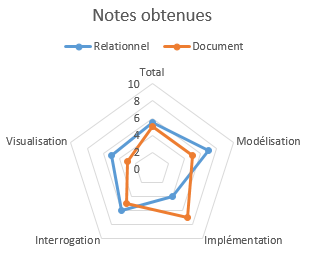
\includegraphics[width=0.5\textwidth]{./src_img/notes.png}
  \caption{Notes obtenues}
  \label{fig:note}
\end{figure}

\paragraph{}Cependant, ce que j'ai pu retenir par rapport au jeu de données choisis, c'est que l'ensemble était riche, bien structuré bien qu'avec quelques colonnes superflus car calculées, mais surtout que les données étaient figées. Dans le contexte actuel, chargé, nombre de sujets auraient pu être choisis dans le cadre de ce mémoire, comme les déplacements de population juste avant ou au début du confinement mais également l'évolution de l'épidémie de COVID-19 sur différentes échelles (locale, nationale, mondiale). Cependant, ces données s'avèrent trop changeantes, elles évoluent tous les jours, et contiennent également des erreurs.


%Je viens de voir les ajouts. Le mémoire maintenant est un peu plus riches, sauf que tu ne mets pas assez en valeur la partie application (en terme de rédaction). Je vais relire le tout en détail et te faire des suggestions.
%Sinon, le paragraphe "Évaluation de mon apport" est à développer. Personnellement j'aurais changé le titre avec "Synthèse et discussion" et enrichir la discussion. Tu expliques que tu as essayé de comparer les deux outils par rapport à 4 points: conception, implémentation, interrogation et visualisation. Ensuite, tu décris pour chaque point ton retour (il faut que ça soit personnalisé) et tu peux même donner une note (seulement par rapport à cette application). Tu peux en finir avec une figure (par exemple figure type radar) pour représenter tes notes.






%\paragraph{}Dans ma proposition, j'ai fait le choix de comparer les deux catégories de bases de données, relationnels et NoSQL, selon des critères liées aux performances. Cela correspond à quelques critères parmi l'infinité de critères possibles. 
%\paragraph{}Afin de mener cette comparaison à bien, je me suis basé sur une source de données commune. L'actualité chargée a permis de générer nombre de jeux de données potentiels : évolution de l'épidémie de COVID-19 à l'échelle locale, nationale ou mondiale, les statistiques liées au confinement telles que les déplacements de population au début de la période, les résultats d'élections. J'ai fait le choix parmi toutes ces possibilités de prendre les résultats du 1\ier tour des élections municipales de mars 2020, les autres jeux de données bougeant constamment et contenant parfois des erreurs. Vis-à-vis du jeu choisi, la totalité des données nécessaires étaient présentes mais d'autres étaient superflues car calculées à partir d'autres.



%début d'année avec corona et élections
%modification des données = plus de complexité
%adapté en fonction de mes ressources et bien sûr avec des ressources adaptées

%implémentation permet de voir les avantages du nosql mais également ces limites avec un si petit ensemble

%améliorations : quantité, structure, etc
%open data : amélioration de la sélection des données et vérification


\chapter{Conclusion}


\paragraph{}Dans ce mémoire, j'ai pu présenter le domaine des \acrfull{SIG} avec ses composants dont les données possèdent une part importante. Nous nous sommes donc tourné sur l'étude du stockage de ces dernières via des bases de données relationnelles ou NoSQL. Cette réflexion a permis de comprendre que le NoSQL est plus adapté aux volumétries toujours plus importantes dans ce domaine.

\paragraph{}Pour compléter cette étude du domaine, un panorama d'outils a été étudié. Tout d'abord ont été vues des solutions intégrant les principes de Codd à l'instar de PostGIS. Ont été également vus les différences entre les \acrshort{SGBD} avec des fonctions géométriques et les outils spécialisés dans le traitement de données géographiques. Par la suite, un zoom sur le NoSQL a été fait avec l'étude de MongoDB. Ce dernier offre de plus grandes libertés vis-à-vis du modèle utilisé. Pour compléter cela, l'étude des technologies de traitement multidimensionnel comme SOLAP et des solutions sur Cloud ont été réalisés.

\paragraph{}Toute cette réflexion a amené à comparer les deux types de bases de données. À partir d'un jeu de données commun, deux modélisations et traitement d'implémentation des modèles ont été proposés. Sur l'ensemble, le modèle doucment obtient une meilleure note que le modèle relationnel. Concernant l'interrogation, les résultats obtenus ont été corrects pour les deux, étant inférieurs à une seconde. Cependant, au vu de la source réduite en fonction des contraintes techniques, il s'avère que le relationnel obtient de meilleurs résultats. Cela vient à confirmer pour les petits jeux de données, le relationnel peut être privilégié.

\paragraph{}Le bilan de ce mémoire vient à confirmer que le type de base de données doit dépendre des besoins techniques comme la volumétrie. Nous avons pu voir par l'application que sur les petits jeux de données bien structurés, le relationnel est à privilégier. Cependant, si on s'engage sur des volumes plus importants, sur un stockage de manière distribué ou sur des formats moins structurés, le NoSQL reste la meilleure solution.




\newpage
%\nocite{SpaceXFirstISS, IFPI2011Report, SpotifyBloomberg, SpotifyNewYorker}

\printbibliography[
heading=bibintoc,
title={Bibliographie}
]
%report and book
\clearpage %\cleardoublepage %for openright
\listoffigures
\clearpage %\cleardoublepage %for openright
\listoftables
\clearpage %\cleardoublepage %for openright

\newpage
\printglossaries

\newpage
\thispagestyle{empty}
\vspace*{\fill}
\begin{center}
  Université Paris-Nanterre\\
  200 Avenue de la République\\
  92000 Nanterre
\end{center}
\vspace*{\fill}

\end{document}